\documentclass[a4paper,11pt,headings=small,headsepline,titlepage,listof=totoc,index=totoc,bibliography=totoc,bibliography=totocnumbered]{scrartcl}
\newcommand{\ThesisAuthor}{Laurenz Anton Dilba}
\newcommand{\ThesisAuthorAddress}{Industriestr. 5 \\ 53721 Siegburg}
\newcommand{\ThesisExternalCompany}{CONET Solutions GmbH}
\newcommand{\ThesisKeywords}{Keywords die diese Arbeit beschreiben}
\newcommand{\ThesisLocation}{Hennef}
\newcommand{\ThesisPubDate}{\today}
\newcommand{\ThesisDateRange}{01. März 2022 bis 22. Mai 2022}
\newcommand{\ThesisSubject}{tests}
\newcommand{\ThesisStudyCourse}{Computer Science}
\newcommand{\ThesisStudyCourseGerman}{Wirtschaftsinformatik}
\newcommand{\ThesisSubjectType}{Bachelorarbeit}
\newcommand{\ThesisSupervisorFirst}{Prof. Dr. Matthias Bertram}
\newcommand{\ThesisSupervisorSecond}{}
\newcommand{\ThesisSupervisorExternal}{Prof. Dr. Wolfgang Heiden}
\newcommand{\ThesisTitle}{Entwicklung einer Schnittstelle für die Anbindung von austauschbaren Datenquellen an KI-Algorithmen}
\newcommand{\ThesisType}{Bachelor}
\usepackage{aussehen/hbrs-inf}
%\usepackage{draftwatermark}
%\SetWatermarkText{Confidential}
%\SetWatermarkScale{5}
%\SetWatermarkText{DRAFT}
%\SetWatermarkColor[gray]{0.95}
%\SetWatermarkFontSize{1.5cm}
\begin{document}
    \begin{spacing}{1}
        \pagenumbering{roman}

        \pagestyle{empty}
        \begin{titlepage}
    \begin{Large}
        \begin{flushleft}
            \makebox[11cm][c]{
                \parbox[c]{2.5cm}{
\includegraphics[height=4ex]{bilder/fhlogo}\vspace{1.40cm}}
                \parbox[c]{12.0cm}{\begin{flushleft}
                                       \small{\textbf{Hochschule\linebreak{}Bonn-Rhein-Sieg}\linebreak{}\textit{University of Applied Sciences}\linebreak{}\linebreak{}\textbf{Fachbereich Informatik}\linebreak{}\textit{Department of Computer Science}}
                \end{flushleft}}}
        \end{flushleft}
    \end{Large}

    \vspace{0.150\textheight}
    \begin{center}
        \begin{huge}
            \textbf{\ThesisSubjectType}
        \end{huge}\\
        \vspace{2em}
        \begin{Large}
            im Bachelorstudiengang \ThesisStudyCourseGerman
        \end{Large}
        \vspace{0.10\textheight}\\
        \begin{huge}
            \textbf{\ThesisTitle}
        \end{huge}\\
        \vspace{2em}
        \begin{Large}
            \textbf{von}
        \end{Large}\\
        \vspace{1em}
        \begin{Large}
        	\begin{spacing}{1.125}
        	\textbf{\ThesisAuthor}
        	\end{spacing}
        \end{Large}
    \end{center}
    \vspace{0.100\textheight}

    \begin{large}
        \begin{flushleft}
            \begin{tabular}{ll}
                Erstprüfer:          & \ThesisSupervisorFirst    \\
                Zweitprüfer: & \ThesisSupervisorExternal \\
                Unternehmen:      & \ThesisExternalCompany    \\
                ~                  &                           \\
                Eingereicht am:    & 9. Januar 2023
            \end{tabular}
        \end{flushleft}
    \end{large}
\end{titlepage}

        \pagestyle{bisHauptteil}
        \input{abschnitte/Erklärung}
        \newpage
        \tableofcontents
        \newpage
        \listoffigures
        \newpage
        \listoftables
        \newpage
        \lstlistoflistings
        \newpage
        \setcounter{secnumdepth}{0}
        \section{Abkürzungsverzeichnis}
\begin{acronym}[DSGVOO]
	\acro{ajax}[AJAX]{Asynchronous JavaScript and XML}
	\acro{amqp}[AMQP]{Advanced Message Queuing Protocol}
	\acro{api}[API]{Application Programming Interface}
	\acro{bert}[BERT]{Bidirectional Encoder Representations from Transformers}
	\acro{bl}[BL]{Business Logic}
	\acro{dsgvo}[DSGVO]{Datenschutz-Grundverordnung}
	\acro{gui}[GUI]{Graphical User Interface}
	\acro{html}[HTML]{Hypertext Markup Language}
	\acro{http}[HTTP]{Hypertext Transfer Protocol}
	\acro{id}[ID]{Identifikation}
	\acro{iec}[IEC]{International Electrotechnical Commission}
	\acro{it}[IT]{Informationstechnik}
	\acro{json}[JSON]{JavaScript Object Notation}
	\acro{jwt}[JWT]{JSON Web Token}
	\acro{ki}[KI]{Künstliche Intelligenz}
	\acro{mac}[MAC]{Message Authentication Code}
	\acro{ram}[RAM]{Random-Access Memory}
	\acro{rdbms}[RDBMS]{relationalen Datenbankmanagementsystemen}
	\acro{rest}[REST]{Representational State Transfer}
	\acro{tcp}[TCP]{Transmission Control Protocol}
	\acro{ui}[UI]{User Interface}
	\acro{url}[URL]{Uniform Resource Locator}
	\acro{uuid}[UUID]{Universally Unique Identifier}
	\acro{vm}[VM]{Virtuelle Maschine}
	\acro{wsl}[WSL]{Windows-Subsystem für Linux}
	
\end{acronym}

        \setcounter{secnumdepth}{3}
        \newpage
      
    \end{spacing}

    \pagestyle{Einleitung}
    \setcounter{page}{1}
    \pagenumbering{arabic}
    \begin{spacing}{1.25}
    
    
    \section{Einleitung}
text
\subsection{Motivation und Hintergrund}
text
\subsection{Problemstellung}
text
\subsection{Aufbau}
text
    \newpage
    
    \pagestyle{Grundlagen}

	\section{Grundlagen}
\subsection{Schnittstelle}
Die Schnittstelle in der Informatik beschreibt sowohl den Bereich einer Software, der nach außen hin für andere Programme oder den Nutzer erreichbar ist, als auch eine eigenständig Anwendung, die zwei unabhängige Programme miteinander verbindet. Innerhalb einer Schnittstelle sind Funktionen vorgegeben, durch die der Nutzer mit der Software interagieren kann. Oftmals werden Schnittstellen für eine spezifische Anwendung entwickelt, um die Nutzung dieser Anwendung zu ermöglichen. Das Ziel einer Schnittstelle ist es, die Komplexität von bestehenden Programmen zu verringern. Der Satz der bereitgestellten Funktionen dient zur Vereinfachung der Bedienung komplizierter oder alter Programme. 
\footcite{sneed2006integrating}

Es wurden zwei Bereiche innerhalb der Schnittstelle entworfen. Der erste Bereich der Schnittstelle verbindet die Website mit dem Backend. Innerhalb des Backends wurde eine Schnittstelle in Form eines \ac{api} implementiert. Der zweite implementierte Bereich der Schnittstelle schließt das Backend mittels RabbitMQ an die einzelnen KI-Services an. In Kapitel 2.2 wird der Aufbau und die Funktionsweise der beiden Schnittstellen genauer erläutert.

\subsection{REST und RabbitMQ}
\subsubsection{Application Programming Interface}
Eine API ist eine Programmierschnittstelle, die dazu da ist, die Kommunikation zwischen einem Client, oder auch Anwender genannt, und einem Server durch festgelegte Funktionen zu regeln. Der Satz der verfügbaren Funktionen ist durch den Entwickler der API vorgegeben. Eine API sollte nach Möglichkeit selbsterklärend aufgebaut sein. \footcite{bloch2006design} Eine API dient dazu, dem Nutzer Daten bereitzustellen oder dem Server Daten zu senden.

In Abbildung 1 ist die Kommunikation zwischen einem Anwender und der API durch ein Sequenzdiagramm dargestellt. Jede Anfrage an die API findet durch den Aufruf des API Endpunkts durch einen \ac{url} statt. Hinter der Grund-URL wird die genaue Ressource innerhalb der API durch den Pfad in der URL angegeben. Jede dieser Funktionen, die über eine bestimmte URL erreichbar sind, kann mehrere Effekte haben. Der Effekt, den eine Funktion hat, ist durch die \ac{http} Methoden im groben Rahmen vorgegeben. Die Kommunikation zwischen API und Anwender geht immer vom Anwender aus. Die API kann den Anwender von sich aus nicht ansprechen. 

\begin{figure}[H]
  \centering
    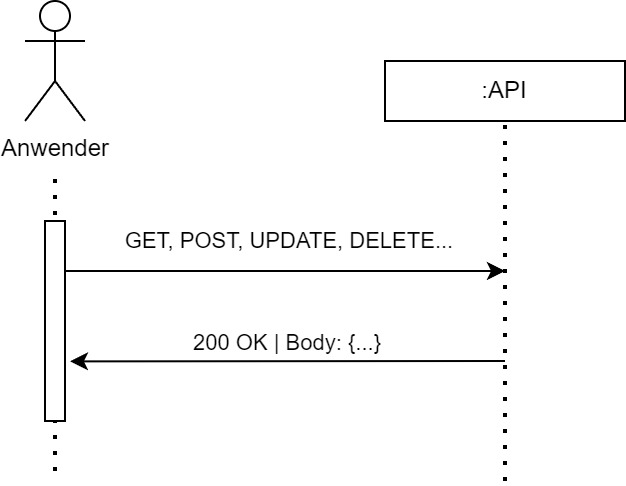
\includegraphics[width = 8cm]{bilder/APISequenzdiagramm}
    \caption{UML Sequenzdiagramm einer API}
\end{figure}

Der gesamte Satz der verfügbaren HTTP-Methoden lautet \texttt{GET, HEAD, POST, PUT, DELETE, CONNECT, OPTIONS, TRACE, PATCH}. Jede der Methoden hat eine bestimmte Aufgabe und bestimmte Rechte, die es vom Entwickler der API einzuhalten gilt.\footcite{mdn2022http} In der Bachelorarbeit werden die Funktionen \texttt{GET, POST} und \texttt{DELETE} verwendet. Routen der API, die mit einer \texttt{GET} Funktion aufgerufen werden, sollen lediglich Daten an den Nutzer zurückgeben, ohne Änderungen auf dem Server vorzunehmen. Wenn zweimal hintereinander die gleiche URL mit \texttt{GET} aufgerufen wird, sollte auch in beiden Fällen das gleiche Ergebnis von der API zurückgegeben werden.

Die \texttt{POST}-Methode liefert Daten vom Nutzer an den Server. Innerhalb des \texttt{POST}-Bodys können Daten im JSON-Format an die API gesendet werden. Neben dem JSON-Format gibt es auch noch weitere Möglichkeiten für Formate. Diese werden in der Bachelorarbeit jedoch nicht behandelt. API URLs, die mit einer \texttt{POST}-Methode aufgerufen werden, können Veränderungen auf dem Server auslösen. Dies kann Auswirkungen auf die Daten oder den Status des Servers haben, sodass andere Methoden eventuell davon beeinflusst werden. Ein beispielhafter Anwendungsfall für eine \texttt{POST}-Methode ist die Registrierung eines neuen Accounts auf einer Website. Dort werden innerhalb des Bodys der Benutzername und das Passwort an die API geschickt. Die API registriert den Account mit den erhaltenen Daten und gibt bei zukünftigen Aufrufen der URL mit den gleichen Daten eine Fehlermeldung zurück, dass der Benutzer bereits registriert ist.

Die \texttt{DELETE}-Methode entfernt eine Ressource unter der aufgerufenen URL. Sowohl bei \texttt{POST} als auch bei \texttt{DELETE}-Methoden ist darauf zu achten, dass der Nutzer die Route nur aufrufen kann, wenn er entsprechende Rechte zur Ausführung verfügt. Ansonsten könnte es zu unkontrollierten Daten- und Statusänderungen innerhalb der API kommen. 

Wie in Abbildung 1 zu sehen ist, gibt die API nicht nur die angeforderten Daten zurück, sondern auch einen Statuscode. Ein HTTP-Statuscode besteht aus drei Ziffern. In Tabelle 1 sind die grundlegenden Statuscodes aufgelistet.

\begin{table}[H]
\centering
\begin{tabular}{l|l}
\textbf{Statuscode} & \textbf{Bedeutung} \\
\hline
1xx & Informationen, nur unter HTTP 1.1 definiert \\
2xx & Request war erfolgreich (OK) \\
3xx & Die Ressource wurde verschoben \\
4xx & Die Eingabe war fehlerhaft \\
5xx & Der Server hatte einen Fehler \\
\end{tabular}
\caption{HTTP Statuscodes nach \cite{doglio2015pro}}
\end{table}

Die Statuscodes, die im Prototyp der Bachelorarbeit verwendet werden, sind Teil der häufiger genutzten Statuscodes für APIs. Der Statuscode \texttt{200:OK} ist der am häufigsten auftretende Statuscode. Dieser besagt, dass die Anfrage erfolgreich abgelaufen ist und das Ergebnis zurückgegeben werden konnte. Der Prototyp nutzt ein Authentifizierungssystem. Dadurch kann es dazu kommen, dass bei einer Anfrage mit fehlender Autorisierung der Statuscode \texttt{401:Unauthorized} zurückgegeben wird. Weitere Statuscodes, die häufiger auftreten können, sind \texttt{404:Not found}, \texttt{405:Method not allowed} und \texttt{500:Internal server error}. Bei einem Statuscode 404 wurde eine Route aufgerufen, die innerhalb der API nicht definiert ist. Bei dem Statuscode 405 wurde zwar eine vorhandene Route angesprochen, jedoch ist die genutzte HTTP-Methode nicht zulässig. Der letzte verwendete Statuscode 500 beschreibt eine fehlerhafte Ausführung der Anfrage. 

Die HTTP-Methoden und Statuscodes dienen dazu, die Entwicklung und Arbeit mit einer API für den Entwickler einfach zu gestalten. Wie die URLs der API aufgebaut sind und welche HTTP-Methoden wann verwendet werden, liegt jedoch vollständig beim Entwickler der API. Um APIs im Allgemeinen etwas zu vereinheitlichen und die Effekte der Funktionen innerhalb der API selbsterklärender werden zu lassen, wurde im Jahr 2000 von Roy Thomas Fielding ein Regelwerk namens \ac{rest} veröffentlicht.\footcite{fielding2000rest}

\subsubsection{Representational-State-Transfer}
REST ist ein Architekturstil, die den Aufbau der Kommunikation im World Wide Web. Der Representational-State-Transfer ist kein spezifischer Standard in der Softwareentwicklung. APIs, die versuchen, den Prinzipien dieses Architekturstils zu folgen, werden als \glqq REST-APIs\grqq{} oder \glqq RESTful-APIs\grqq bezeichnet. Diese bieten damit einen größtenteils standardisierten Weg, Daten zwischen Client und Server auszutauschen. \footcite{richards2006representational}

Innerhalb des REST-Frameworks sind mehrere Aspekte vorgegeben, die eine REST-API ausmachen. Drei der Aspekte sind Simplizität, Skalierbarkeit und Performance. Die Simplizität beschreibt einen allgemeinen, standardisierten Weg, wie der Aufbau und die Kommunikation mit der API ablaufen soll. Dies beinhaltet den Aufbau der Routen und damit der URL, wann Daten an die API geschickt werden sollen, sowie die Form der Daten, die zu versenden sind. 

Die Skalierbarkeit beschreibt das Konzept der beliebigen Erweiterung einer API. Das beinhaltet die Entwicklung der API als solche. Routen und damit Möglichkeiten, Daten von der API anzufordern oder Daten an die API zu senden, können während der Entwicklung einfach hinzugefügt und entfernt werden. Das Konzept der Skalierbarkeit beschreibt ebenfalls einen zustandslosen Aufbau der API. Durch die Zustandslosigkeit kann die API horizontal skaliert werden. Eine horizontale Skalierung beschreibt das Hinzufügen neuer Instanzen der API. Jede Instanz ist identisch aufgebaut und kann jede ankommende Anfrage alleinstehend beantworten. Die Anfragen, die an eine REST-API gestellt werden, müssen daher sämtliche für die Bearbeitung notwendigen Informationen bereitstellen.

Der letzte Aspekt des REST-Frameworks beschreibt die Performance. Eine REST-API implementiert ein System zum Zwischenspeichern, Caching gennant, von Responses. Wenn ein Client eine Anfrage mit der HTTP-Methode GET an die API schickt, wird die Antwort, die an den Client zurückgesendet wird, auf dem Server zwischengespeichert. Sollte ein oder mehrere Clients eine identische Anfrage an die API senden, wird das zwischengespeicherte Ergebnis zurückgegeben, statt die dahinter liegende Methode innerhalb der API neu auszuführen. Das ermöglicht eine hohe Performance, auch bei einer großen Anzahl von Anfragen.\footcite{masse2011rest}

\subsubsection{RabbitMQ}
Kommunikation ist für den Aufbau von komplexen Strukturen essenziell. Bei einer Kommunikation gibt es grundsätzlich zwei Beteiligte: Sender und Empfänger. Im Bereich der Software ist der Sender meist ein Client und der Empfänger ein Server, der öffentlich erreichbar ist. Der Client sendet eine Anfrage, der auch Request genannt wird, an den Server. Anschließend wartet der Client auf eine Antwort. Der Server erhält den Request und verarbeitet ihn. Es wird abhängig vom Request eine Antwort, die als Response bezeichnet wird, generiert und dem Client zurückgesendet. Der Client erhält die Response und schließt damit den Kommunikationsvorgang ab. Dieser Ablauf ist in Abbildung 2 visualisiert.

\begin{figure}[H]
  \centering
    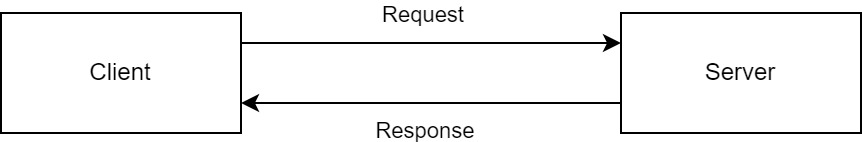
\includegraphics[width = 12cm]{bilder/Rabbit1}
    \caption{Grundlegende Kommunikation}
\end{figure}

Durch die synchrone Kommunikation sind Client und Server eng miteinander verbunden. Der Client erwartet eine Response von dem Server, an den er den Request geschickt hat. Die synchrone Kommunikation erhöht die Komplexität der Skalierung und Ausfallsicherheit.

Damit eine Kommunikation zwischen unabhängigen Programmen möglich wird, muss es einen Zwischendienst geben, der die Nachrichten von einem Programm zum anderen transportiert. Bei der Kommunikation zwischen einer Website und einer API wird das HTTP verwendet. Dieses stellt sicher, dass die die Nachrichten erfolgreich beim Empfänger ankommen. Sollte eine Nachricht nicht angekommen sein, hat der Absender die Möglichkeit, die Nachricht erneut zu schicken. Über HTTP wird automatisch eine erneute Anfrage geschickt, wenn keine Antwort vom Server zurückkam. Problematisch wird diese Herangehensweise, wenn die Antwortzeit sehr lang wird oder ungewiss ist, ob überhaupt eine Antwort kommen wird. Des Weiteren kann es zu Problemen führen, wenn sehr viele Nachrichten zur gleichen Zeit beim Server eintreffen. Der Server versucht sämtliche eingehenden Nachrichten gleichzeitig anzunehmen und zu verarbeiten. Dadurch entsteht eine sehr hohe temporäre Last. Sollte der Server seine Ressourcen, wie CPU oder RAM nicht dynamisch hochskalieren können, führen die eingehenden Anfragen zu einer Überlastung und damit zum Absturz des gesamten Servers.\footcite{hoque2015botnet} Um dies zu verhindern, muss ein Zwischendienst implementiert werden, der die eingehenden Nachrichten annimmt, zwischenspeichert und zum passenden Zeitpunkt weiterleitet, wenn der Server die erforderlichen Kapazitäten zum Verarbeiten einer neuen Anfrage hat.

RabbitMQ ist ein eine im Jahr 2007 veröffentlichte, nachrichtenorientierte Middleware, die eine Kommunikation zwischen zwei oder mehreren Programmen durch das \ac{amqp} ermöglicht. RabbitMQ implementiert einen Broker, der Nachrichten von mehreren Clients an mehrere Server vermitteln kann. Im Gegensatz zu einer direkten Kommunikation zwischen Client und Server wie bei HTTP, wird in RabbitMQ eine Queue implementiert, in der sämtliche Anfragen gesammelt werden.\footcite{JohanssonLovisa2020REBD} In Abbildung 3 ist die Kommunikation zwischen Client und Server mittels eines Brokers abgebildet.
 
\begin{figure}[H]
  \centering
    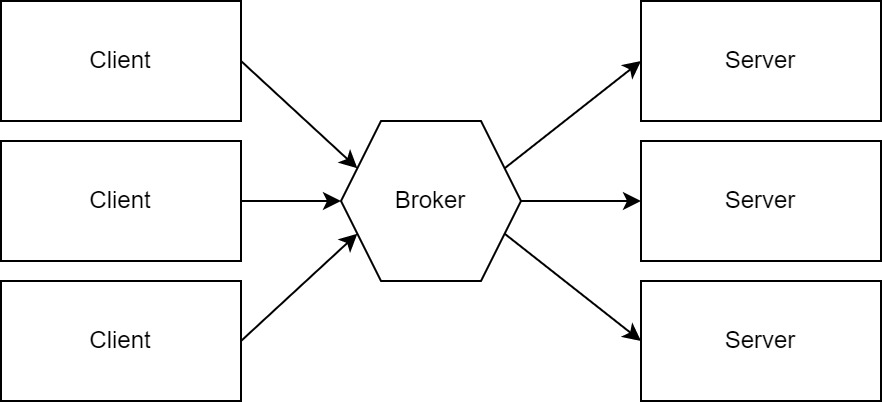
\includegraphics[width = 12cm]{bilder/Rabbit2}
    \caption{Kommunikation über einen Broker nach Dossot}
\end{figure}

Durch diese Herangehensweise wird eine asynchrone Kommunikation zwischen Client und Server ermöglicht. Sollte ein Server oder ein Client während seiner Laufzeit abstürzen, hat dies keine Auswirkungen auf die anderen Instanzen. Des Weiteren kann die Anzahl der Clients und Server, abhängig von der aktuellen Nutzlast, dynamisch hoch- und runterskaliert werden. Eine weitere Eigenschaft, die durch diese Architektur entsteht, ist, dass der Client keine Information darüber besitzen muss, wo sich der Server befindet, oder mit welcher Technologie er implementiert wurde. Solange der Server die Schnittstelle zum Broker implementiert, können die Nachrichten vom Client empfangen werden.\footcite{dossot2014rabbitmq}

Das AMQP ist ein offener Standard, der den Nachrichtenaustausch zwischen Produzent und Konsument regelt. AMQP definiert den gesamten Ablauf des Austausches. Innerhalb des Protokolls wird definiert, wie die \ac{tcp} Verbindung zwischen Client und Broker aufgebaut wird. Ebenfalls Bestandteil des Protokolls ist der softwareseitige Aufbau der Nachrichtenübermittlung. AMQP implementiert mehrere Konzepte, die auch im Prototyp verwendet wurden. Die folgende Aufteilung der Konzepte wurde durch Johansson und Dossot beschrieben.\footcite{JohanssonLovisa2020REBD}

Der Broker ist das grundlegende Konzept von AMQP. Er empfängt Nachrichten von einer Anwendung und leitet sie an eine andere Anwendung weiter.

Der Virtual-Host, genannt vhost, bietet eine Möglichkeit mit mehreren Anwendungen auf dem gleichen Broker zu arbeiten, jedoch ohne dass die Anwendungen Einfluss aufeinander nehmen können. Der vhost bietet eine logische Trennung der Anwendungen innerhalb der gleichen RabbitMQ Instanz.

Eine Connection beschreibt die physische Verbindung zwischen einer Anwendung und dem Broker. Die Verbindung zwischen Anwendung und Broker wird mittels TCP hergestellt. 

Ein Channel ist eine virtuelle Verbindung innerhalb einer Connection. Sendet ein Client eine Nachricht an einen Broker, wird dafür eine virtuelle Connection aufgebaut, statt jedes Mal eine neue TCP-Verbindung zu nutzen. Innerhalb einer Connection können mehrere Channels aufgebaut und genutzt werden. Dadurch können auch mehrere Anfragen über die gleiche TCP Verbindung abgearbeitet werden. 

Ein Exchange hat die Aufgabe, die Nachrichten zwischen Anwendung und Broker zu vermitteln. Der Exchange stellt sicher, dass die Nachrichten ankommen und in die richtige Queue geschrieben werden. In welcher Queue die Nachrichten landen, ist abhängig von den Regeln, die durch den Exchange Typen definiert werden.  

Eine Queue ist eine Datenstruktur, in der mehrere Operationen definiert werden. Die Queue fungiert als Warteschlange, in der Einträge gespeichert und in der Reihenfolge des Eingangs wieder ausgelesen werden. Sie funktioniert nach dem First In - First Out, kurz FIFO, Prinzip. Es wird eine \texttt{push} Operation definiert, mit der ein Eintrag an den Anfang der Warteschlange geschrieben wird. Des Weiteren gibt es eine \texttt{pop} Operation, die das älteste Element aus der FIFO-Queue ausliest und es aus der Warteschlange entfernt. Jeder Client kann Nachrichten in die Queue schreiben. Diese Nachrichten werden dort so lange gespeichert, bis sie von einem Dienst ausgelesen werden. 

Binding beschreibt eine virtuelle Verbindung zwischen einem Exchange und einer Queue innerhalb des Brokers. Diese Verbindung ermöglicht Nachrichtenfluss von einem Exchange zu einer Queue.

In Abbildung 4 sind die Konzepte von AMQP und deren Ablauf visualisiert.

\begin{figure}[H]
  \centering
    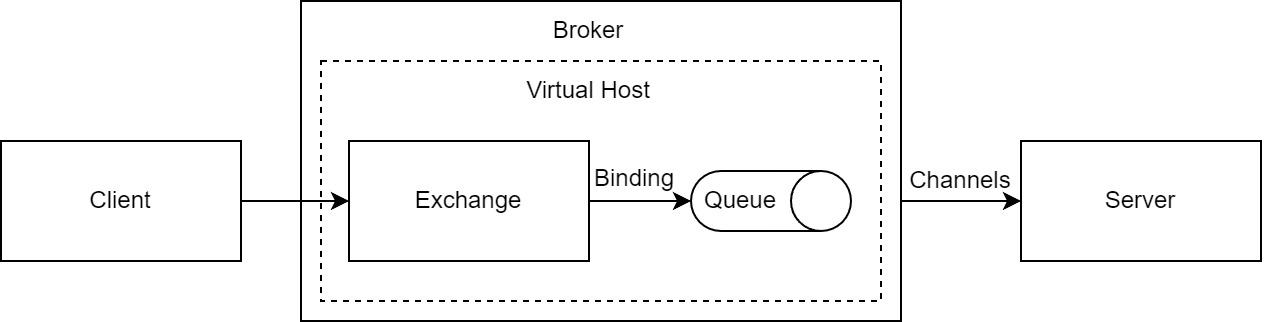
\includegraphics[width = 15cm]{bilder/Rabbit4}
    \caption{Darstellung der AMQP Konzepte nach Dossot}
\end{figure}

Die Middleware RabbitMQ wird im Prototyp für die Kommunikation zwischen der Flask API und den KI-Services genutzt. Sowohl das Backend, in dem die API implementiert ist, als auch die einzelnen KI-Services sind als Teil einer Microservice-Architektur implementiert. RabbitMQ wird als universelle Schnittstelle für die Kommunikation in der Microservice-Architektur verwendet. 

\subsection{Microservice-Architekturen}
Das Konzept von Microservices beschreibt die Unterteilung einer umfangreichen Anwendung in einzelne Teilanwendungen. Eine Teilanwendung wird dabei Microservice genannt. Die einzelnen Teilanwendungen sollen dabei untereinander kommunizieren können, um die Zusammenarbeit zu gewährleisten. Dazu nutzen die Teilanwendungen eine universelle Schnittstelle. Eine Anwendung soll nur eine Aufgabe erledigen. Der Umfang dieser Aufgabe ist nicht genauer definiert.\footcite{wolff2018microservices}

Die Idee von Microservices ist es, ein großes System in viele kleine einzelne Systeme aufzuteilen. Dadurch entsteht eine Modularisierung der einzelnen Services. Voneinander unabhängige Softwaremodule können im Gegensatz zu einem Softwaremonolithen unabhängig voneinander deployed werden. Dies ermöglicht es zur Laufzeit bestimmte Teile des Softwaresystems hoch- und runterzufahren. Ein Austausch von fehlerhaften Services oder das Dazuschalten von neuen Services bei mangelnder Leistung ist, während das Softwaresystem in einer Produktivumgebung genutzt wird, möglich.\footcite{newman2015microservices}

Jedes Teilsystem kann einzeln deployed werden. Dadurch kann die Verfügbarkeit des gesamten Systems gewährleistet werden, auch wenn bestimmte Bereiche der Software aktualisiert oder verändert werden müssen. Bei einem Monolithen müsste für jede Änderung am System die gesamte Anwendung heruntergefahren und neugestartet werden.  

Microservices sind voneinander unabhängige Programme und damit auch eigenständige Prozesse. Die Technologie, mit der ein Service implementiert wird, ist nicht durch die allgemeine Architektur oder das System vorgegeben. Jeder Service kann in der für ihn passenden Technologie und Programmiersprache entwickelt werden. 

Da die Technologien der Services unabhängig voneinander sind, muss es eine gemeinsame Schnittstelle zur Kommunikation geben. Über diese Schnittstelle werden Daten und Information ausgetauscht, die die jeweiligen Services zum Bearbeiten ihrer Aufgaben benötigen. Die Kommunikation im Prototyp wird mit RabbitMQ implementiert. 

\subsection{Künstliche Intelligenz}
Der Begriff KI beschreibt eine Software, die das Ziel hat, typisch menschliche Aufgaben, wie Sehen, Hören und Verstehen von Kontext abzubilden.\footcite{gorz2010handbuch} 
KIs benötigen eine große Menge an Daten als Grundlage, mit denen sie trainiert werden können. Ein nicht trainiertes KI-Modell kann nicht viel mehr als zufällige Entscheidungen treffen. Erst durch das Training bekommen die Entscheidungen der KI eine Struktur. Nachdem eine KI für ihren bestimmten Einsatzzweck mit den entsprechenden Daten trainiert wurde, kann sie verwendet werden. Die Verwendung einer KI folgt den Grundprinzipien eines normalen Algorithmus. Es wird ein Input angenommen, wie beispielsweise ein Text oder ein Bild. Dieser wird durch die KI analysiert und in eine für die KI verständliche Form gebracht.\footcite{hamet2017artificial} Diese Form ist im Falle des Prototyps ein 512-dimensionaler Vektor. Anschließend generiert die KI einen Output. Dieser kann das Endergebnis der Anfrage sein oder für weitere Verarbeitungsschritte genutzt werden.

KIs können von Grund auf selbst entwickelt und trainiert werden. Die Anwendungszwecke einer KI überschneiden sich jedoch oftmals mit bereits vorhandenen Modellen, die es frei oder gegen eine Nutzungsgebühr auf dem Markt gibt. Wenn eine fertig trainierte KI genutzt werden kann, spart dies Entwicklungszeit und Ressourcen. Die vortrainierten KIs werden jedoch meist als Blackbox angeboten. Eine Blackbox ist ein geschlossener Raum, der eine Eingabe annimmt und eine Ausgabe produziert, ohne dass der Nutzer der Blackbox sehen kann, wie der Algorithmus funktioniert, der zu der Ausgabe führt.  

Ein KI-Service beschreibt eine Implementierung einer solchen Blackbox. Ein KI-Service ist ein alleinstehendes Programm, das die Aufgabe hat, Nachrichten anzunehmen, sie zu transformieren, zu analysieren und anschließend ein oder mehrere Ergebnisse zurückzugeben. 

Um die Nachrichten empfangen und die Ergebnisse zurücksenden zu können, muss in jedem Service eine Schnittstelle implementiert sein, über die die Nachrichten empfangen werden können. Innerhalb des Prototyps wird in den einzelnen KI-Services RabbitMQ als Schnittstelle genutzt.

Im Prototyp zur Anbindung von austauschbaren Datenquellen an KI-Algorithmen ist ein Service zur Textähnlichkeitssuche implementiert. Dieser nutzt das \ac{bert}-Modell von Google. Dieser Service ermöglicht die semantische Suche in einer Datenbank. Nicht-KI-gestützte Textsuchalgorithmen können in einer Datenbank lediglich nach übereinstimmenden Wörtern oder Wortteilen suchen. Wenn ein Nutzer sämtliche Einträge zu einem bestimmten Thema aus der Datenbank herausfiltern möchte, muss die passenden Schlüsselwörter kennen, die in den Datenbankeinträgen vorhanden sind. Sucht man in einer Datenbank beispielsweise nach \glqq JavaScript\grqq{} und es gibt nur Artikel, die die Abkürzung \glqq JS\grqq{} beinhalten, liefert die Suche keine Ergebnisse. Eine gewisse Textähnlichkeit kann erreicht werden, wenn zum Beispiel Leerzeichen oder Groß/Kleinschreibung ignoriert werden. 

Eine Textänlichkeitssuche, die mittels KI durchgeführt wird, kann zu einer Anfrage wie \glqq JavaScript\grqq{} deutlich mehr Ergebnisse liefern. Sie ist nicht durch die in der Suche angegebenen Zeichen beschränkt, sondern versucht den Inhalt der Anfrage zu verstehen. Anschließend kann in der Datenbank nach inhaltlich ähnlichen Artikeln gesucht werden, die zur Anfrage passen. Der \glqq verstandene\grqq{} Satz, der für die Suche in der Datenbank genutzt wird, ist abhängig vom verwendeten KI-Modell. Für die Textähnlichkeitssuche im Prototyp wird das BERT Modell von Google verwendet, um die Anfrage in einen 512-dimensionalen Vektor zu konvertieren. Jede Dimension des Vektors wirkt sich auf die Interpretation des Vektors aus. Der Vektor wird daher auch als \glqq dense vector\grqq{}, oder auch dichter Vektor bezeichnet. Damit die Suche über den Vektor funktioniert, wird ein zweiter Vektor benötigt, mit dem der, durch die Suchanfrage erzeugte, Vektor verglichen werden kann. Jeder Eintrag in der Datenbank muss daher einmalig mit dem gleichen KI-Modell analysiert werden. Der jeweils erzeugte Vektor wird in der Datenbank abgespeichert, um ihn für kommende Suchanfragen nutzen zu können.

Der Grundsatz des KI-Modells ist es, dass zwei Sätze, die inhaltlich ähnlich sind, auch zwei ähnliche Vektoren besitzen. Vektoren sind ähnlich, wenn der Abstand der beiden gering und die Richtung ähnlich ist.\footcite{rahutomo2012semantic} Diese Abstandsberechnung kann in der Elasticsearch Datenbank seit Version 7.3, welche am 31.07.2019 veröffentlicht wurde, automatisch durchgeführt werden. 

\subsection{Verwendete Werkzeuge}
\subsubsection{Python API mit Flask}
%Implementierung der Rest api durch Flask
Python ist eine um 1991 von Guido van Rossum entwickelte Programmiersprache. Bei der Entwicklung von Python wurde ein besonderer Fokus auf die Lesbarkeit von Code gesetzt. Dank der simplifizierten Syntax im Vergleich zu anderen höheren Programmiersprachen wie Java oder C\#, ist Python auch in Bereichen, wie in der Mathematik oder der Wissenschaft ein häufig genutztes Werkzeug. Python bietet ebenfalls die Möglichkeit, von anderen Entwicklern bereitgestellte Bibliotheken in das eigene Projekt zu integrieren.\footcite{python2021python} 

Flask ist eine der verfügbaren Bibliotheken, die ein Framework für die Implementierung einer webbasierten API bereitstellt. Eine API dient dazu, Funktionen und Routen zu definieren, um die Kommunikation zwischen dem Frontend und dem Backend herzustellen. Das Flask-Framework ist im Gegensatz zu anderen Frameworks sehr klein. Dies ermöglicht ein schnelles aufsetzen und entwickeln. Da Flask nur die nötigsten Grundlagen für eine API mitliefert, ist der Code besser lesbar und damit für andere Entwickler besser wartbar.\footcite{grinberg2018flask} 

Die Flask-API wird für die Anbindung des Frontends an die Datenbank, sowie die Anbindung an die Kommunikationsschnittstelle von RabbitMQ verwendet. Sie nimmt die Daten oder die Eingaben des Nutzers entgegen und vermittelt sie an den richtigen Dienst, damit sie von einer KI-Schnittstelle ausgewertet werden können. Anschließend kann die API angefragt werden, ob es bereits Antworten von einer KI zu der vorher geschickten Anfrage gab. Falls die API die Auswertung der KI erhalten hat, wird diese für das Frontend bereitgestellt, um sie dort anzeigen zu können.  

\subsubsection{REDIS und MySQL-Datenbanken}
Redis ist eine In-Memory Key-Value-Datenbank. Im Gegensatz zu \ac{rdbms} wie MySQL oder PostgreSQL werden in Redis keine festen Tabellenstrukturen hinterlegt. Redis gehört damit zur Kategorie der NoSQL-Datenbanken (Not Only SQL). Key-Value-Stores sind kein Ersatz für eine relationale Datenbank, bieten aber für bestimmte Bereiche große Vorteile. Durch das Fehlen von komplexen Strukturen innerhalb der Datenbank kann Redis Anfragen weitaus schneller als andere Datenbanksysteme bearbeiten. Da Redis im \ac{ram} ausgeführt wird,  werden die Daten grundsätzlich nicht persistent gespeichert. ACID (Atomicity, Consistency, Durability and Isolation) Konformität wird mit Redis ebenfalls nicht gewährleistet. Für den Einsatzzweck als Cache in einer Cloud-Umgebung ist Redis allerdings sehr gut geeignet. \footcite{paksula2010persisting}

Innerhalb des durch Redis implementierten Key-Value-Stores werden sämtliche relevanten Daten gespeichert, die ein Nutzer während seiner Benutzung der Software produziert. Dort werden ebenfalls die Zwischenergebnisse abgespeichert, die die KI während der Analyse erstellt.
%
%\subsection{MySQL Datenbank für Services und Logs}
MySQL ist ein um 1995 erschienenes Open-Source RDBMS. MySQL ist eines der weitverbreitetsten und schnellsten Datenbanksysteme in seiner Kategorie. \footcite{dubois2008mysql}

In relationalen Datenbanken werden Daten strukturiert in Tabellenform abgespeichert. Einzelne Tabellen können Verlinkungen und Referenzen auf andere Tabellen haben, damit die Zusammengehörigkeit der Daten beschrieben werden kann, ohne Daten redundant speichern zu müssen. In MySQL, wie auch anderen RDBMS, werden Tabellenstrukturen und Daten persistent abgespeichert. In-Memory-Datenbanken wie Redis können Daten über Umwege auch persistent speichern, jedoch müssen dafür größere Anpassung an der Konfiguration von Redis vorgenommen werden.

Das RDBMS MySQL wird u. a. für die Speicherung der Logs, die der Flask-Server während der Verarbeitung von Requests oder Nachrichten an die KI produziert, verwendet. Ein weiterer Einsatzzweck der MySQL-Datenbank ist die Speicherung der im System registrieren KI-Services. Ein Dienst kann über die Flask-API im System registriert oder deregistriert werden. Das Frontend kann im Anschluss eine Auflistung der verfügbaren Services beim Backend anfragen.

\subsubsection{Angular Frontend}
Eine Website wird üblicherweise mit \ac{html} und JavaScript erstellt. Um eine moderne Website zu entwickeln, die ihren Inhalt nicht beim ersten Aufrufen lädt, sondern erst dann, wenn er benötigt wird, müssen Konzepte wie \ac{ajax} verwendet werden. Angular ist ein von Google entwickeltes und gepflegtes Open Source-Framework, zur Vereinfachung des Entwickelns von komplexen webbasierten Anwendungen. Angular bietet im Gegensatz zu anderen Webframeworks wie React und Vue.js eine vollumfängliche Bibliothek, mit der nahezu sämtliche Aspekte in der Web-Entwicklung abgedeckt werden können.\footcite{moiseev2018angular}

In Angular wird die Programmiersprache TypeScript verwendet. Diese ist eine Erweiterung der Programmiersprache JavaScript und implementiert Konzepte wie feste Typisierung von Variablen. Weitere Konzepte wie Dependency-Injection oder die Trennung von \ac{bl} und \ac{ui} ermöglichen eine schnelle Entwicklung von komplexen Systemen. 

Das Frontend wird für die Ein- und Ausgabe der Daten verwendet. Der Nutzer kann auf der Webseite seine Suchanfrage in ein Textfeld schreiben und anschließend auf den Server hochladen. Im nächsten Schritt wird die Möglichkeit bereitgestellt, die eingegebenen Daten automatisiert zu bearbeiten und zu manipulieren. Im gleichen Zug wird die Eingabe des Nutzers in ein für die KI verständliches Format konvertiert. Im letzten Schritt schickt der Nutzer die Anfrage an das Backend, mit der Analyse der Eingabe zu beginnen. Das Frontend fängt daraufhin an, beim Backend in regelmäßigen Abständen nach Antworten der KI zu fragen. Antworten werden in einer Liste visualisiert.

\subsubsection{Logging durch Grafana}
Grafana ist ein von Torkel Ödegaard in 2014 entwickeltes Open-Source-Datenvisualisierungsprogramm. Grafana kann zeitbasierte Daten durch verschiedene Arten von Grafen und Diagrammen anzeigen.\footcite{chakraborty2021grafana}

Eines der möglichen Panels für ein Dashbaord ist das Log-Panel. Dort werden die Log Nachrichten aus einer Datenbank angezeigt und mit einer Farbe, abhängig vom Schweregrad markiert. Als Datenquelle können u. a. zeitbasierte Datenbanken z. B. InfluxDB und Prometheus oder RDBMS wie MySQL verwendet werden.

Im implementierten Prototyp wurde eine MySQL verwendet, in der die zu loggende Nachricht, der Schweregrad, der Zeitstempel und die User-\ac{id} gespeichert werden. Diese Daten werden verwendet, um die Logs im Log-Panel von Grafana chronologisch anzeigen zu lassen.

\subsubsection{Deployment über Docker}
Docker ist eine Software zur Isolierung von Anwendungen mithilfe von Containervirtualisierung. Ein Container beschreibt eine in sich geschlossene Umgebung, in der ein Programm ausgeführt werden kann. Die benötigten Dateien, Parameter und Umgebungsvariablen werden beim Starten des Containers mitgegeben. Damit wird sichergestellt, dass ein innerhalb eines Docker-Container ausgeführten Programms sich in jeder Umgebung gleich verhält. Hierdurch wird die Unabhängigkeit vom Host-Betriebsystem gewährleistet. Im Gegensatz zu einer \ac{vm} muss für die Ausführung eines Docker-Containers kein komplettes Betriebssystem virtualisiert werden. Das Hochfahren einzelner Container ist schneller und ressourcenschonender als die Implementierung einzelner VMs.\footcite{anderson2015docker} Des Weiteren können über das Docker-Compose-Plugin mehrere Container gleichzeitig hochgefahren werden, sodass mit einer einzigen Kommandozeileneingabe eine komplette Softwarearchitektur hochgefahren werden kann.

Docker wird für das Deployment der einzelnen Komponenten des Prototyps verwendet. Für Redis, MySQL, RabbitMQ, Grafana und Elasticsearch können die benötigten Images, die eine Bauanleitung darstellen, aus dem Docker-Hub heruntergeladen und genutzt werden. In einem Docker-Image sind sämtliche für die Ausführung des Programms benötigten Dateien gepackt. Docker-Hub ist eine Plattform zur Verteilung von offiziellen Docker-Images, von der automatisch die Images runtergeladen werden, die lokal nicht vorhanden sind.

Für das Angular-Frontend und das Flask-Backend müssen die Images manuell gebaut werden, bevor sie als Container gestartet werden können. Dafür bietet Docker sogenannte Docker-Files an, in der die benötigten Konfigurationen hinterlegt werden.


	\newpage
	
	\pagestyle{Methodik}	
	
    \section{Methodik}
text
\subsection{Wasserfallmodell}
text\footcite{FrauchigerDaniel2017AvDS}
\subsection{Evaluationsmethode}
text
	\newpage
	
	\pagestyle{Konzeption und prototypische Umsetzung}
	
    \section{Konzeption und prototypische Umsetzung}
In diesem Kapitel wird die prototypische Implementierung der Schnittstelle für die Anbindung von austauschbaren Datenquellen an KI-Algorithmen beschrieben. Zunächst werden die Anforderungen für das Projekt innerhalb der Bachelorarbeit erläutert. Anschließend wird das erarbeitete Konzept beschrieben. Der mithilfe des Konzeptes entwickelte Prototyp sowie das anschließende Deployment findet sich ebenfalls in diesem Kapitel wieder.  

\subsection{Anforderungen}
Die Anforderungen für die Schnittstelle und den daraus resultierenden Prototyp wurden in Zusammenarbeit mit der CONET Solutions GmbH erhoben. Die Projektidee entstand im Kontext eines Projektes zu \glqq Trendscouting Systemen\grqq{}. Das Ziel des Systems sollte es sein, eine Architektur bereitzustellen, die vom Nutzer gestellte Anfragen annimmt und diese mit einer KI analysiert, um Aussagen darüber treffen zu können, welche Technologien in der Zukunft relevant werden könnten. Da der Umfang eines Trend-Scouting Systems zu groß für den Zeitraum einer Bachelorarbeit ist, ergab sich als Zielsetzung die Entwicklung der Architektur, die ein solches System unterstützen könnte. Die genaue Anforderungserhebung wurde nach dem Leitfaden der von der \ac{iec} veröffentlichten Norm IEC 62304 Kapitel 5.2 entworfen.\footcite{daniel2018anforderungen} Innerhalb dieser Norm ist spezifiziert, wie Anforderungen an eine Software aufbereitet und dokumentiert werden sollen.

Im ersten Schritt wurden die Benutzerschnittstellen spezifiziert. Die grundlegende Interaktion mit dem System findet über die Website statt. Dort hat der Nutzer die Möglichkeit seine Suchanfrage in Form eines ausgeschriebenen Satzes oder über einzelne Stichpunkte in ein Textfeld einzugeben. Die nächste Benutzerschnittstelle ist die Transformation der zuvor eingegebenen Suchanfrage. Der Nutzer soll dort mittels JSON-Syntax die Suchanfrage modifizieren können. Dies ist im Hinblick auf eine eventuell automatisierte Nutzung des Systems erforderlich. Im dritten Schritt soll der Nutzer die Option haben, die Suchparameter für die KI anzupassen. Vor allem relevant ist die Anzahl der Ergebnisse, die bei einer gestellten Suchanfrage zurückgegeben werden. An dieser Stelle soll aber auch weitere Parameter eingegeben werden können. Anschließend ist eine Möglichkeit vorgesehen die Anfrage inklusive der Parameter abzuschicken. In Abbildung 5 ist die Interaktion mit dem System in einem Use Case Diagramm dargestellt.

\begin{figure}[H]
  \centering
    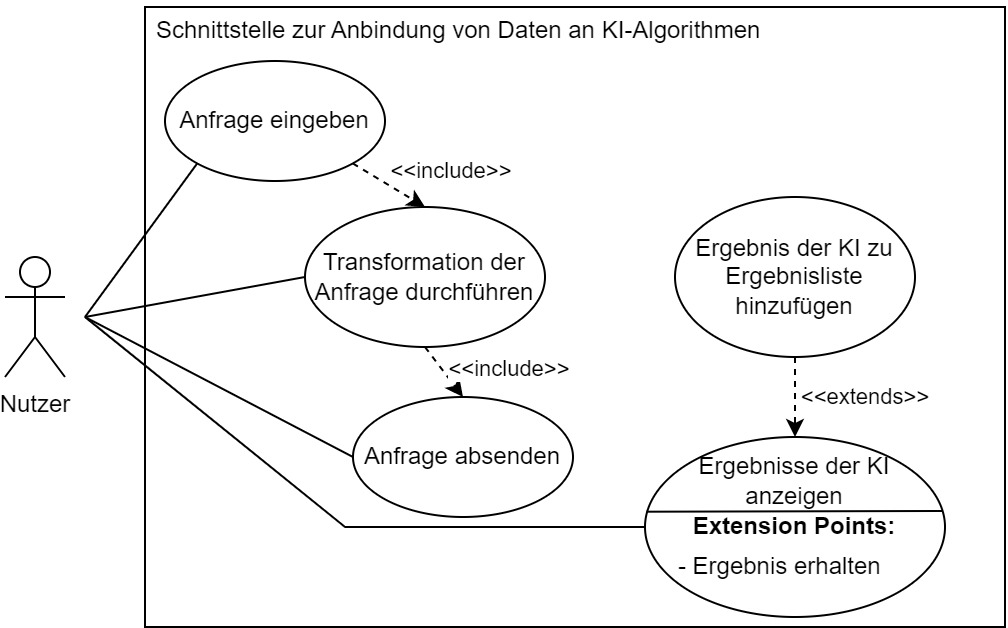
\includegraphics[width = 15cm]{bilder/UseCase}
    \caption{Use Case Diagramm der Interaktion mit der Schnittstelle}
\end{figure}

Die letzte Möglichkeit, die der Nutzer hat, mit der Schnittstelle zu interagieren, ist über die API selbst. Dort gibt es eine Route, über die die aktiven KI-Services verwaltet werden können. Abhängig von der gewählten HTTP-Methode sollen verschiedene Funktionen angeboten werden. Die drei Hauptfunktionen sind die Auflistung aller aktiven Services, das Erstellen eines neuen Services und das Löschen eines Services.

Der nächste Schritt der Anforderungsanalyse nach IEC 62304 ist die Festlegung des \ac{gui}. Die grafische Oberfläche sollte sich auf eine Seite beschränken und in drei Bereiche eingeteilt sein. Jeder der Bereiche beinhaltet eine Kachel mit einer Überschrift. Die drei Überschriften \glqq Query\grqq{}, \glqq Transformation\grqq{} und \glqq Service\grqq{} sollen verdeutlichen, welche Aktionen in der entsprechenden Kachel passieren.
Der linke Bereich der Seite für die Query beinhaltet die Eingabe durch den Nutzer, welche durch ein Textfeld realisiert wird. Des Weiteren gibt es einen Button zum Hochladen der Anfrage an den Server.

Im mittleren Bereich der Seite befindet sich die Kachel für die Transformation der Eingabe. Der Inhalt der Kachel selber ist nochmal in drei Bereiche aufgeteilt. Der erste Bereich zeigt die vom Nutzer hochgeladene Eingabe. In diesem Feld kann der Nutzer keine Änderungen vornehmen. Das zweite Feld enthält die Eingabe für die Transformation. Das Textfeld enthält einen vorgefertigten Text in JSON-Syntax, den der Nutzer anpassen kann. Unter dem Textfeld gibt es einen Button, der die Funktion hat, die Transformationsanleitung an den Server zu senden. Im dritten Feld wird das Ergebnis der Transformation angezeigt, damit der Nutzer überprüfen kann, ob das erzeugte Ergebnis seinen Erwartungen entspricht. 

Der rechte Bereich der Seite ist für die Auswahl und Nutzung der KI-Services vorgesehen. Der gewünschte Service soll über ein Dropdown ausgewählt werden. Da die Services für ihre Anfragen Parameter übergeben bekommen müssen, muss eine Tabellenstruktur implementiert werden. Die Tabelle hat zwei Spalten und beliebig viele Reihen. Innerhalb der Tabelle können Schlüssel-Wert Paare eingegeben werden, wobei der Schlüssel in der ersten Spalte und der Wert in der zweiten Spalte steht. Unter der Tabelle muss es einen Button geben, der die Anfrage an den KI-Service sendet. Daraufhin startet der Abfrageprozess der die Antworten der KI-Services zusammenträgt. Die Ergebnisse des KI-Services werden in einem Feld unter dem Button angezeigt. Bei jedem Ergebnis wird zunächst nur die Überschrift angezeigt. Erst bei einem Klick auf die Überschrift soll der Inhalt ausgeklappt werden.

Der Schritt nach der Anforderungserhebung der grafischen Oberfläche ist die Dokumentation des Verhaltens des Systems. Besonderer Fokus liegt hierbei auf dem Verhalten gegenüber Nutzerinteraktionen. Beim ersten Besuch der Website, wird dem Nutzer ein Token zugesendet, welches für alle weitere Anfragen zur Authentifizierung an der API genutzt werden soll. Innerhalb des Tokens ist eine eindeutige User-ID hinterlegt. Nachdem der Nutzer auf der linken Seite der Website in der Kachel \glqq Query\grqq{} den Upload Button gedrückt hat, sendet die Website den eingegebenen Text an die API. Dabei soll im Authorization Header der Token stehen und im Request Body der eingegebene Text in JSON-Syntax. 

Ist die Anfrage beim Server eingegangen, soll sie in einem Redis Cache hinterlegt werden und anschließend wieder ans Frontend zur Bestätigung zurückgesendet werden. Sollte bei der Anfrage ein Fehler aufgetreten sein, wird der Statuscode 500 an die Website zurückgegeben und das Ergebnis des Uploads wird nicht im ersten Feld der Transformation angezeigt. Sollte der Upload erfolgreich gewesen sein, wird der Text dort angezeigt und der Nutzer hat die Möglichkeit, eine Transformationsanleitung in JSON-Syntax einzugeben und diese über den \glqq Transform\grqq{} Button an das Backend zur Auswertung zu schicken. Die Transformationsanleitung wird, nachdem sie im Backend eingetroffen ist, ebenfalls im Redis Cache gespeichert. Das Backend führt eine Transformation mit der gegebenen Anleitung durch und sendet sie zurück an die Website. Das Ergebnis der Transformation wird im dritten Feld der \glqq Transformation\grqq{} Kachel angezeigt. Bei einem Fehler während der Transformation wird der Statuscode 500 zurückgesendet und es werden keine Ergebnisse angezeigt.

In der \glqq Service\grqq{} Kachel im rechten Bereich der Seite kann der Nutzer über ein Dropdown einen von allen aktiven Services auswählen. Die Liste der Services wird beim Laden der Seite von der API angefragt. Die API stellt dafür eine SQL Anfrage an eine MySQL Datenbank, in der alle aktiven Services hinterlegt sind. Anschließend kann der Nutzer einen oder mehrere Parameter in einer Tabelle eingeben. Der ausgewählte Service und die eingegebenen Parameter werden durch den Klick auf einen \glqq Execute\grqq{} Button unterhalb der Tabelle an die API gesendet. Das Backend soll die transformierten Anfragen über RabbitMQ an den dafür vorgesehenen Service schicken. Zur Bestimmung des Services wird der mitgelieferte Servicename genutzt, der durch die Dropdownauswahl ermittelt wird. Jede einzelne Anfrage soll eine Anzahl an erwarteten Antworten haben. Das Backend teilt die Gesamtzahl der erwarteten Antworten der Website mit, wo sie zur Anzeige für den Nutzer verwendet werden kann. 

Der zu implementierende Service ist eine Textähnlichkeitssuche. Dieser Service erhält die vom Backend gesendeten Anfragen und dazu soll mittels des BERT-Modells die semantisch ähnlichsten Texte aus einer Elasticsearch Datenbank herausfiltern. Die ähnlichsten Texte werden über RabbitMQ wieder an das Backend gesendet, wo sie im Redis Cache zwischengespeichert werden. Die Website soll nach dem Absenden der Anfrage in regelmäßigen Intervallen Anfragen an die API stellen, ob Antworten vom KI-Service im Backend eingetroffen sind. Bei einer solchen Anfrage schaut das Backend im Redis Cache nach, ob eine oder mehrere Antworten existieren. Falls dies der Fall sein sollte, sendet die API die Antworten. Im Fall, dass noch keine Antworten im Redis Cache liegen, gibt das die API eine Antwort mit der Nachricht \texttt{successful:False} zurück. Die Website stellt so lange Anfragen an die, bis die erwartete Zahl der Antworten eingetroffen ist.

Der nächste Punkt in der IEC 62304 ist die Festlegung der Geschwindigkeit, in der das System bestimmte Aufgaben abarbeiten soll. Hierzu gab es bezüglich der KI-Services keine genaue Vorgabe seitens der CONET. Das Backend und die Kommunikation zu den einzelnen Service hatte jedoch gewisse Maximallaufzeiten. Eine Anfrage, die durch einen HTTP-Request in der API ankommt, soll maximal 0,5 Sekunden benötigen, um an den richtigen Service weitergeleitet zu werden. Die Rückrichtung vom Service zum Backend soll ebenfalls maximal 0,5 in Anspruch nehmen. Die Gesamtzeit der Kommunikation zwischen Backend und einem Service darf demnach nicht mehr als eine Sekunde betragen. Da der KI-Algorithmus keine festgelegte Laufzeit hat, soll durch die Architektur, mit der die Systeme aufgesetzt sind, kein großer zusätzlicher Overhead entstehen. Antwortzeiten innerhalb einer Sekunde gelten laut der CONET als responsiv und praxistauglich.

In der Spezifikation IEC 62304 wird ebenfalls gefordert, die Umgebung, in der die Software installiert werden soll, zu definieren. Die Hauptanforderung der CONET war hierbei, dass das System möglichst plattformunabhängig entwickelt werden soll. Für die Installation der einzelnen Komponenten ist Docker vorgesehen.

Der letzte festgehaltene Punkt aus der IEC 62304 ist die Beschreibung, wie das System auf  Benutzerfehler und Überlast reagieren soll. Grundsätzlich sollen Benutzerfehler im Backend abgefangen werden und nicht zum Serverabsturz führen. Dazu soll ein System implementiert werden, was potentielle Fehler abfängt und anschließend in eine MySQL Datenbank logged. Des Weiteren sollen alle aufgerufenen Routen und Vorgänge innerhalb des Backends, sowie den einzelnen Services geloggt werden. Dadurch kann nachvollzogen werden,  ob das System ordnungsgemäß funktioniert. Die Architektur soll horizontal skalierbar sein. Das bedeutet, dass mehrere Instanzen der API und der einzelnen Services parallel betrieben werden können. Jede dieser Instanzen muss für sich allein stehend voll funktionsfähig sein.

\subsection{Konzeption}
\subsubsection{Softwarearchitektur}
Ein grundlegender Dienst, der Daten mit einer KI verbindet, kann mithilfe eines einzigen Python-Scripts erstellt werden. Die Herausforderung an einer praxistauglichen Anwendung, die gleichzeitig von mehreren Usern genutzt werden kann, liegt im  Architekturdesign der Software. Eine praxistaugliche Anwendung muss neben den funktionalen Anforderungen auch noch weitere nicht funktionale Anforderungen erfüllen. Laut der CONET sind die drei wichtigsten nicht funktionalen Anforderungen Performance, Skalierbarkeit und Verfügbarkeit. Alle drei Anforderungen können mit einem lokal ausgeführten Skript nicht erfüllt werden. 

Damit Nutzer mit der Software interagieren können, wird ein Frontend benötigt. Ein zentral gehostetes, webbasiertes Frontend kann von einem Nutzer über eine einfache URL im Webbrowser aufgerufen werden. Für die anzuzeigenden Daten im Frontend wird eine Verbindung zum Backend benötigt. Diese wird über eine HTTP Verbindung zur mit Flask gehosteten REST API bereitgestellt.

Um die Anforderung der Skalierbarkeit erfüllen zu können, ist die REST-API komplett zustandslos implementiert worden. Eine API ohne Zustände speichert keine Zwischenstände zu den Anfragen einzelner Nutzer. Bei jeder Anfrage an die API müssen alle Informationen im Request bereitgestellt werden, die die API zum Bearbeiten der Anfrage benötigt. Dies bietet die Möglichkeit bei steigender Nutzerzahl mehrere parallel betriebene Instanzen der API hochzufahren. Dadurch ist eine horizontale Skalierung gewährleistet. Horizontal skalierbare Instanzen innerhalb der Softwarearchitektur sind in Abbildung 6 mit zwei hintereinander gestapelten Rechtecken visualisiert.

Da die Kommunikation zwischen dem Frontend, der API und den KI-Services asynchron läuft, muss das Flask Backend trotz seiner Zustandslosigkeit Transformationsanleitungen und Ergebnisse der KI-Services zwischenspeichern, bis sie im Frontend benötigt werden. Um die Performanceanforderungen erfüllen zu können, können nicht alle Zwischenstände in einer MySQL Datenbank gespeichert werden. Die Lese- und Schreibgeschwindigkeit kann bei steigender Nutzerzahl problematisch werden. Um dem Entgegenzuwirken, wird ein Redis Key-Value Store als Cache betrieben. Die zwischengespeicherten Daten werden nach dem ersten Aufruf wieder gelöscht, weswegen eine persistente Speicherung nicht notwendig ist. In-Memory Datenbanken speichern und führen ihre Queries direkt im RAM aus, wodurch Anfragen im Vergleich zu einer MySQL Datenbank deutlich schneller ausgeführt werden.

Im Flask Backend werden alle Routen und die meisten Funktionen abgekapselt in einem Funktion Wrapper ausgeführt. Dieser fungiert als eine Art Sandbox, in der auftretende Fehler nicht zum Programmabsturz führen, sondern behandelt und geloggt werden können. Alle Logs werden persistent in einer MySQL Datenbank gespeichert. Mit dem Dienst Grafana können diese Logs angezeigt werden.

Die Laufzeit von KI-Services kann sehr stark vom verwendeten KI-Modell, der zu durchsuchenden Datenmenge, wie auch der vom Nutzer gesendeten Eingabe abhängen. Bei einer synchronen Kommunikation zwischen dem Flask Backend und dem Service können sehr lange Wartezeiten entstehen. Wenn der KI-Service ebenfalls eine REST-Schnittstelle implementieren würde, könnten es bei einem HTTP Request zum Timeout der Anfrage führen. Aufgrund der schwanken Laufzeit muss eine asynchrone Kommunikationsstruktur, wie RabbitMQ mit dem AMQP implementiert werden.

Die einzelnen Services können mit einem Eintrag in der MySQL Datenbank registriert werden. Für die Registrierung muss lediglich der Name und der im Frontend anzuzeigende Name des Services hinterlegt werden. Die Registrierung eines Dienstes kann durch den Aufruf einer Route in der API durchgeführt werden. 

Der im Prototyp implementierte KI-Service nutzt das BERT Modell von Google zum Konvertieren der Nutzereingaben in semantische Vektoren. Es wird ebenfalls eine Elasticsearch Datenbank betrieben, in der alle zu Durchsuchenden Einträge gespeichert sind. Im Gegensatz zu einer MySQL Datenbank, kann in einer Elasticsearch Datenbank zu jedem Eintrag ein semantischer Vektor gespeichert werden. Der KI-Service kann mithilfe der Kosinusähnlichkeitssuche den semantischen Vektor der Eingabe mit den Vektoren der Datenbank vergleichen und so die semantisch ähnlichsten Texte herausfiltern. Die gefunden Einträge werden über RabbitMQ im Anschluss wieder an das Flask Backend geschickt, damit sie dort vom Frontend ausgelesen werden können.

\begin{figure}[H]
  \centering
    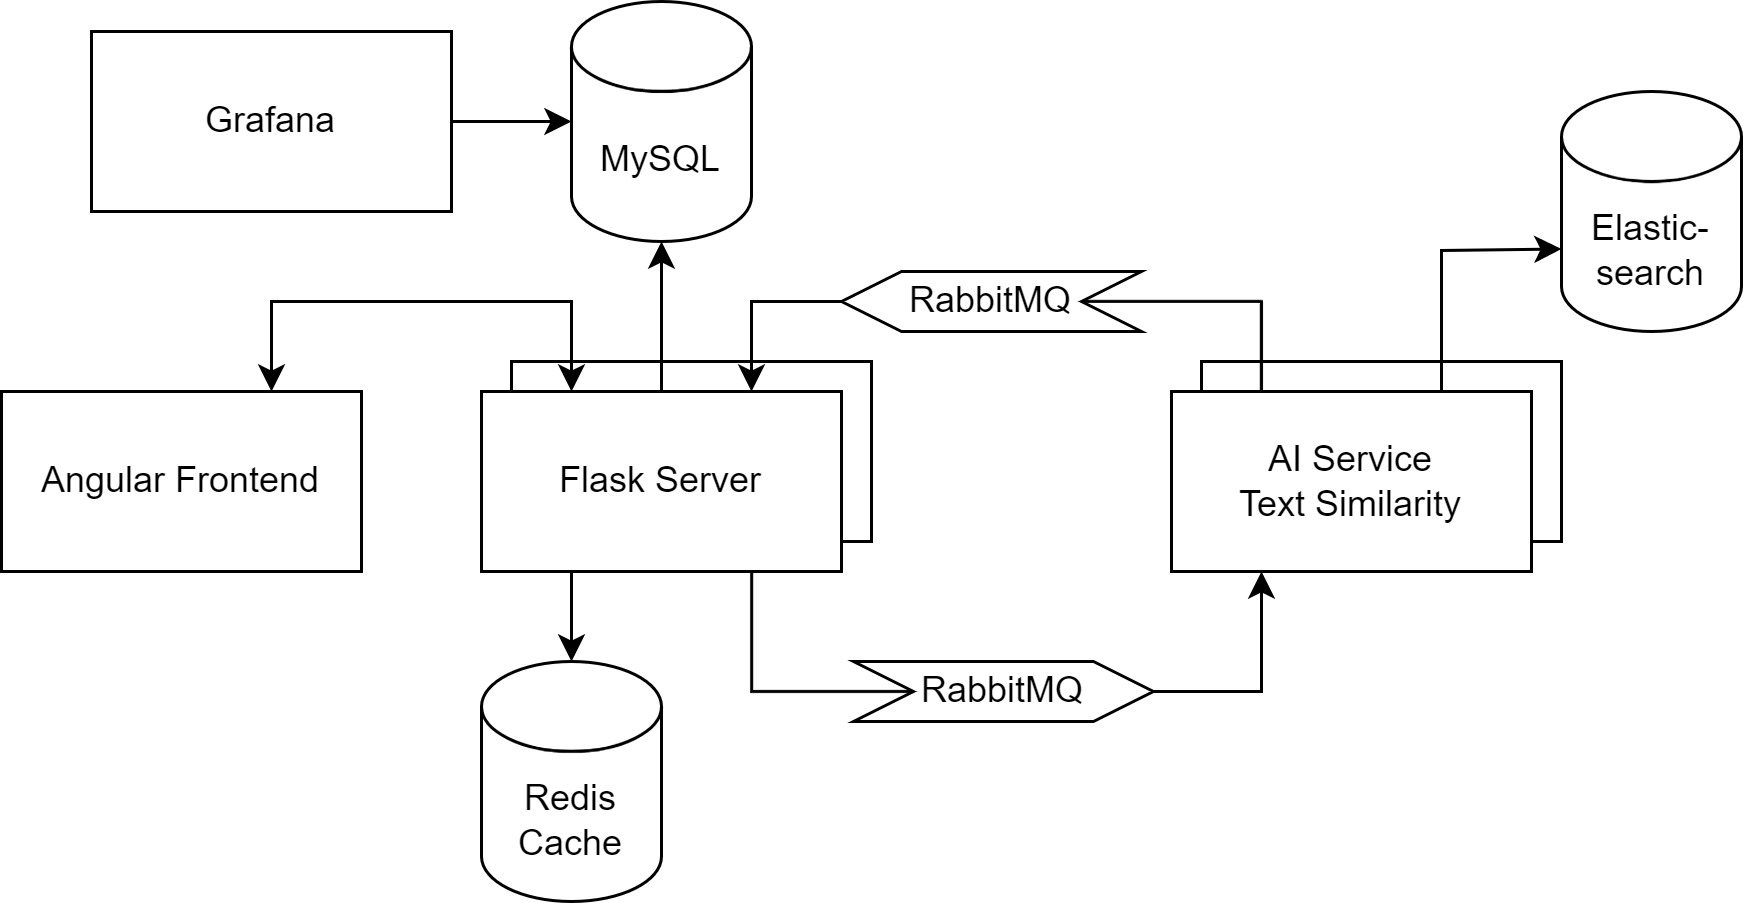
\includegraphics[width = 12cm]{bilder/Architektur}
    \caption{Softwarearchitekturdiagramm}
\end{figure}

\subsubsection{Programmablauf}
\begin{figure}[H]
  \centering
    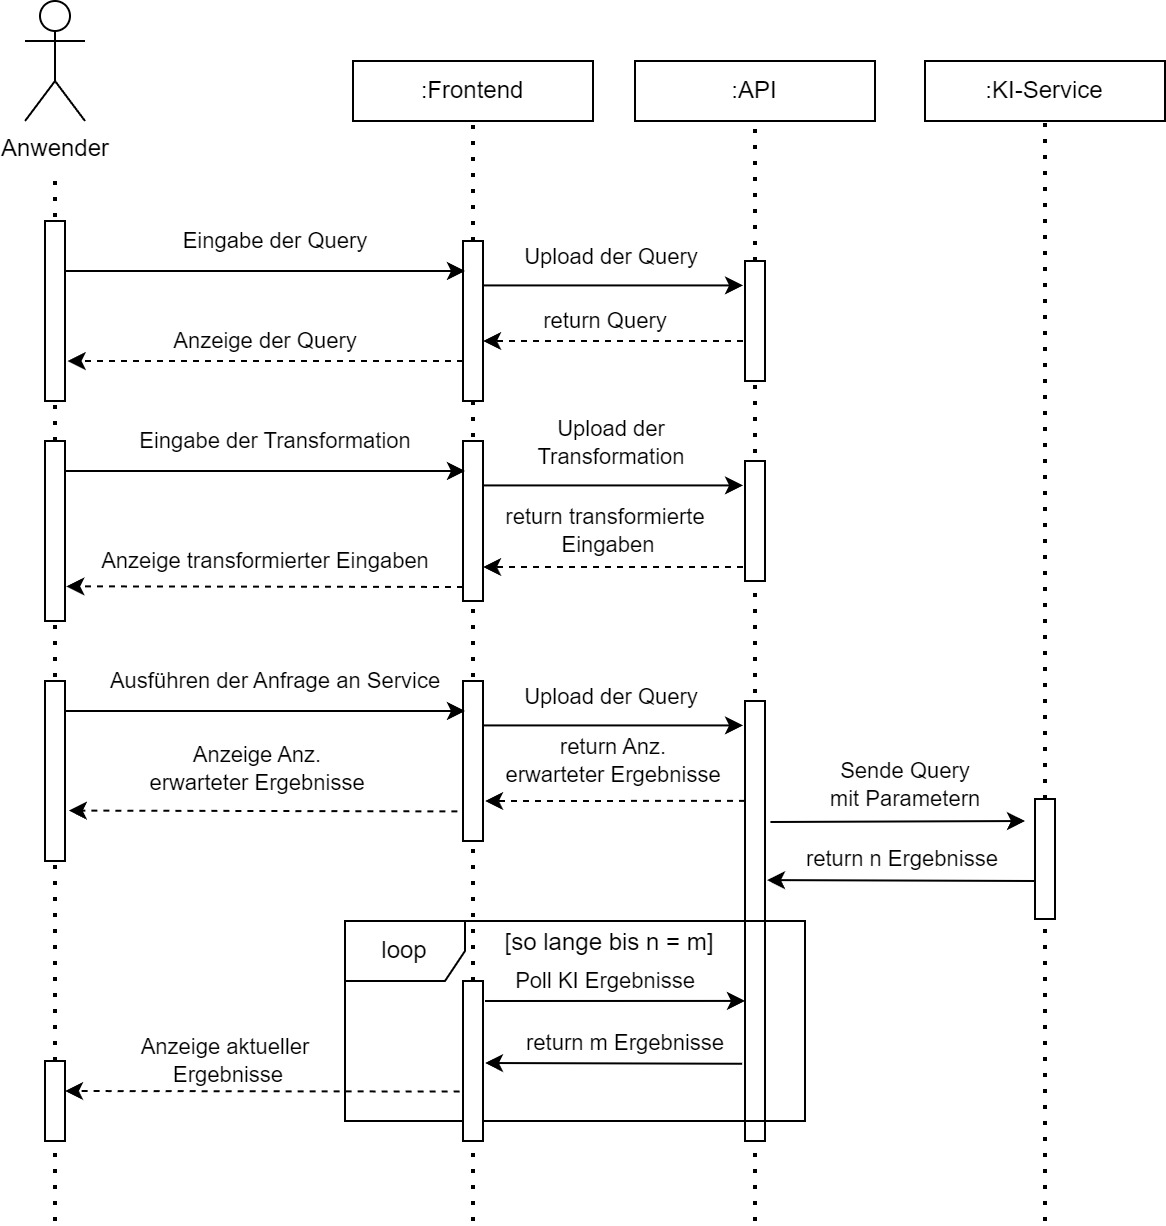
\includegraphics[width = 15cm]{bilder/ArchitekturSequenz}
    \caption{UML Sequenzdiagramm des Programmablaufs}
\end{figure}

Das Ziel der Bachelorarbeit ist es, eine Schnittstelle zu entwickeln, die Daten an KI-Algorithmen anbindet. Dazu wird im Prototyp ein System implementiert, welches die Anbindung in drei Schritten durchführt. In Abbildung 7 ist der grundlegende Programmablauf in einem UML Sequenzdiagramm dargestellt. In Abbildung 8 ist ein Mockup der gesamten Website abgebildet. Alle Interaktionen, die der Anwender auf der Website tätigen kann, sind hier beispielhaft abgebildet. Die Mockups dienen der Veranschaulichung des entwickelten Konzepts für die Nutzerinteraktion mit der Schnittstelle. 

\begin{figure}[H]
  \centering
    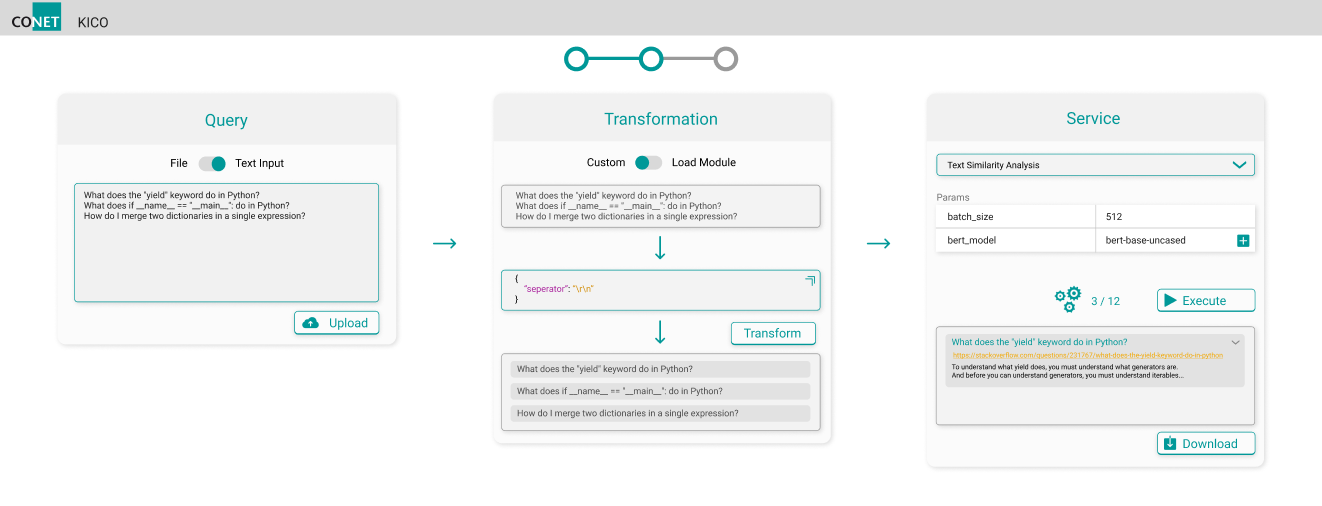
\includegraphics[width = 15cm]{bilder/mockup}
    \caption{Mockup Frontend}
\end{figure}

Der erste Schritt ist, wie auch in den Anforderungen definiert, die Eingabe der Query durch den Anwender. Auf der Website gibt es dafür ein Textfeld, in dem diese Eingabe stattfindet. Eine Darstellung der \glqq Query\grqq{} Kachel ist in Abbildung 9 gegeben. Die Eingabe kann durch einen Klick auf den \glqq Upload\grqq{} Button an die API per HTTP POST-Request geschickt werden. Innerhalb des Bodys befindet sich die Eingabe. Zusätzlich zu dem Body wird ein Authorization Header mitgeschickt, der die User-ID des Anwenders enthält. Innerhalb der API wird die User-ID als Schlüssel und die Qeury als Wert für einen Eintrag in den Redis Cache genutzt. Die Eingabe wird im Backend zunächst nur zwischengespeichert. Als Bestätigung für den Nutzer, sendet die API die erhaltene Query wieder an die Website zurück. Dort wird sie im oberen Bereich der \glqq Transformation\grqq Kachel angezeigt. 

\begin{figure}[H]
  \centering
    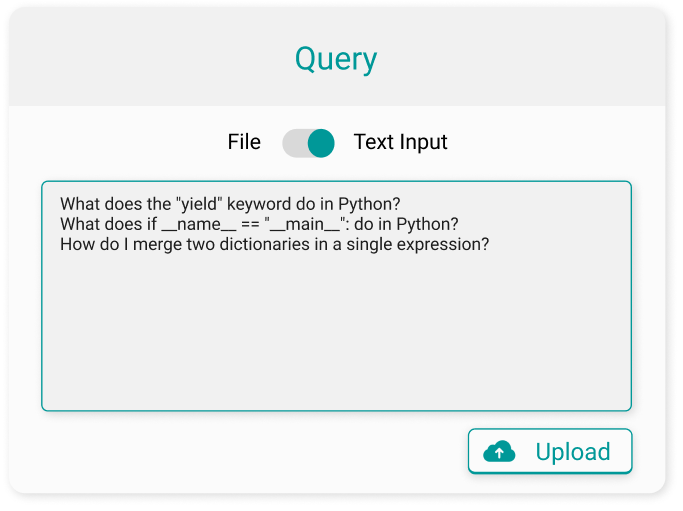
\includegraphics[width = 10cm]{bilder/mockupQuery}
    \caption{Mockup Query}
\end{figure}

Der zweite Schritt ist die Eingabe der Transformationsanleitung. In Abbildung 10 ist das Mockup für die \glqq Transformation\grqq{} Kachel abgebildet. Im mittleren Textfeld der \glqq Transformation\grqq{} Kachel ist für diesen Schritt ein Textfeld vorgesehen. Nach Abschluss der Eingabe kann der Anwender auf den Button \glqq Transform\grqq{} klicken, um die Eingabe an die API hochzuladen. Wie auch bei dem Upload der Query wird die User-ID im Header des Requests mitgeschickt. Die API nutzt die User-ID um die zuvor hochgeladene Query aus dem Redis Cache zu laden. Die im Request mitgelieferte Transformationsanleitung wird in diesem Schritt genutzt, um die Query zu transformieren. Im Prototyp wird eine Split-Operation beliebige Anzahl an Replace-Operationen implementiert. Die Split-Operation teilt die Query in mehrere einzelne Queries. Dazu wird eine Zeichenkette genutzt, die als Trennzeichen dient. Die Replace-Operation ersetzt eine eingegebene Zeichenkette durch eine andere. Das Ergebnis der Transformation wird innerhalb der Response wieder an die Website gesendet. Sollte eine Split-Operation angegeben worden sein, werden alle daraus resultierenden Queries im unteren Bereich der \glqq Transformation\grqq{} Kachel angezeigt. 

\begin{figure}[H]
  \centering
    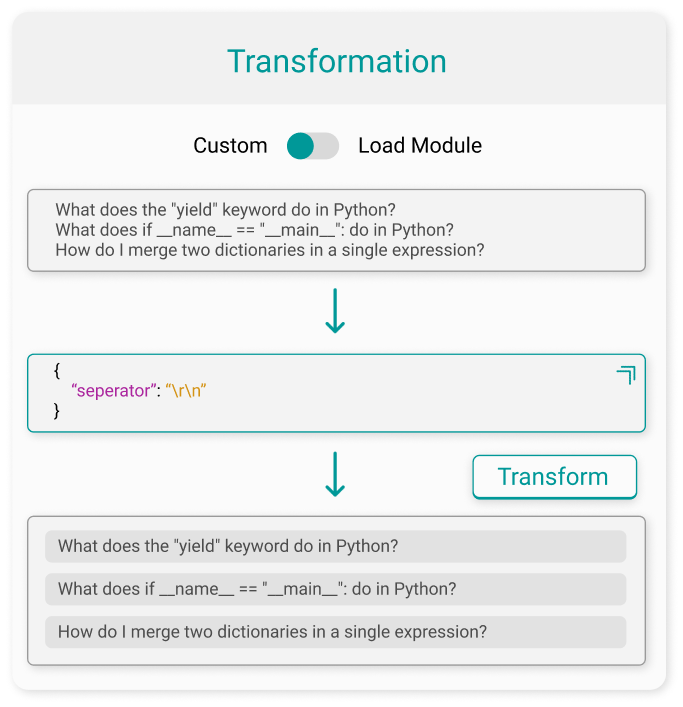
\includegraphics[width = 10cm]{bilder/mockupTransformation}
    \caption{Mockup Transformation}
\end{figure}

Der dritte Schritt ist die Ausführung der Anfrage durch einen KI-Service. In Abbildung 11 ist das Mockup für die \glqq Service\grqq Kachel dargestellt. Der Anwender  wählt im Dropdown der Kachel \glqq Service\grqq{} einen der in der MySQL Datenbank hinterlegten aktiven Services aus und gibt anschließend einen oder mehrere Parameter in die Tabelle unterhalb des Dropdowns ein. Durch einen Klick auf den Button \glqq Execute\grqq{} wird eine Query im Frontend zusammengebaut und als Request an die API gesendet. Innerhalb der Query befindet sich der Name des KI-Services, sowie alle in der Tabelle definierten Parameter. Wenn der Request bei der API eingegangen ist, lädt das Backend sowohl die in Schritt eins eingebene Query, sowie die in Schritt zwei eingegebene Transformationsanleitung. Das Backend führt nun eine erneute Transformation durch und sendet dem Frontend die Anzahl der erwarteten Antworten des KI-Services zurück. Die Anzahl setzt sich aus der Menge der durch die Split-Operation entstandenen Queries und den eingegebenen Parametern zusammen. Für den KI-Service zur Textähnlichkeitssuche gibt es den Parameter \texttt{search\_{}size}. Die Anzahl der erwarteten Antworten wird im Frontend zunächst zur Fortschrittsanzeige genutzt. Der zweite Einsatzzweck der erwarteten Antworten ist innerhalb der darauffolgenden Schleife. Nach dem Upload der Query startet die Website eine Schleife in der bei der API regelmäßig nach neuen Ergebnissen des KI-Services gefragt wird. Der KI-Service bekommt direkt nach dem Upload der Query über RabbitMQ die Anfrage zugesendet. Innerhalb des Services in dem die Textähnlichkeitssuche  implementiert wird, wird die eingehende Nachricht angenommen und mithilfe des BERT-Modells in einer Elasticsearch Datenbank nach den semantisch ähnlichsten Einträgen gesucht. Es werden, abhängig von der \texttt{search\_{}size}, die ähnlichsten Ergebnisse gesammelt und über RabbitMQ wieder an das Backend gesendet. Im Sequenzdiagramm in Abbildung 7 ist die Anzahl mit der Variable \texttt{n} angegeben. Die Ergebnisse werden in einem Redis Cache zwischengespeichert. Wie zuvor erwähnt, läuft parallel zu der Bearbeitung der Services im Frontend eine Schleife, die die Ergebnisse aus der API abfragt. In einer Schleifeniteration werden alle im Redis Cache hinterlegten Ergebnisse aus dem KI-Service abgefragt und an das Frontend gesendet. Die maximale Anzahl der Ergebnisse ist dabei \texttt{m}. Die Schleife läuft so lange, bis die Anzahl der erhaltenen Antworten identisch mit Anzahl der erwarteten Antworten ist, also bis $n=m$ ist. Jedes erhaltene Ergebnis wird im Frontend im unteren Bereich der \glqq Service\grqq{} Kachel angezeigt. Damit ist der Programmablauf abgeschlossen und der Anwender kann eine neue Query eingeben.

\begin{figure}[H]
  \centering
    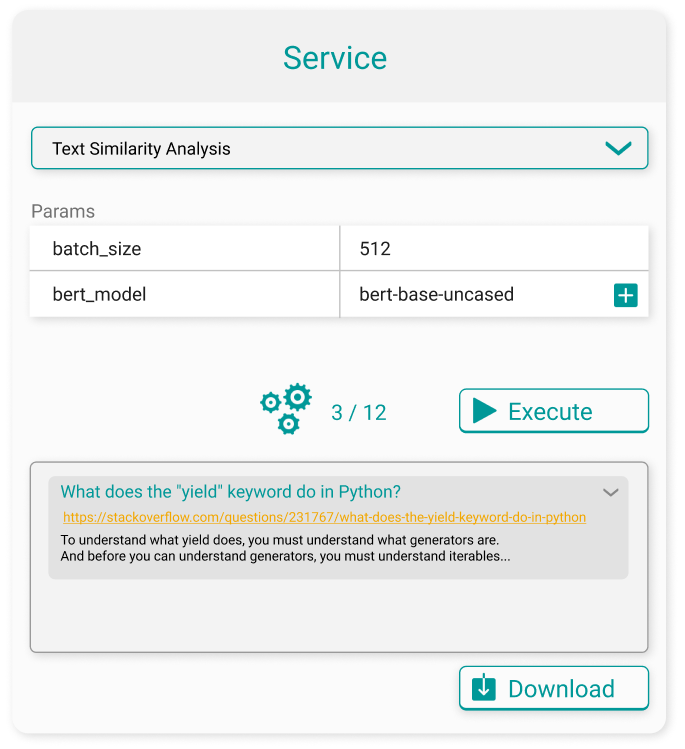
\includegraphics[width = 7.5cm]{bilder/mockupService}
    \caption{Mockup Service}
\end{figure}

\subsection{Prototypische Umsetzung}
\subsubsection{Implementierung der REST-API}
Python bietet mit dem Package Flask die Möglichkeit einen simplen und gut skalierbaren Webserver aufzusetzen. Für das Starten einer Flask-Instanz muss das Package Flask in die Python Umgebung importiert werden. Anschließend kann ein Flask-Objekt erzeugt und die Flask-Instanz mit den gewünschten Parametern gestartet werden.

\begin{lstlisting}[language=Python, caption={Aufsetzen einer Flask-Instanz}]
from flask import Flask
app = Flask(__name__)
app.run(host="0.0.0.0", port=80, use_reloader=False)
\end{lstlisting}

Damit die API auch automatisiert aus einem Docker Container heraus gestartet werden kann, muss die Ausführung des Flask Services in die Main Methode von Python ausgelagert werden. Flask blockiert den Thread, auf dem es ausgeführt wird, was eine asynchrone Kommunikation über RabbitMQ nicht möglich macht. Der Receiver benötigt seinen eigenen Thread, weswegen eine Multithreading-Architektur implementiert werden muss. Zu diesem Zweck wird das threading Package genutzt. Über den Parameter \texttt{daemon} kann bei der Erzeugung eines Threads festgelegt werden, dass der Thread im Hintergrund läuft und den Hauptthread nicht blockiert.

\begin{lstlisting}[language=Python, caption={Flask im eigenen Thread starten}]
def start_server():
    app.run(host="0.0.0.0", port=80, use_reloader=False)

if __name__ == '__main__':
    thread_server = threading.Thread(target=start_server, daemon=True).start()
\end{lstlisting}

Eine in der API adressierbare Route kann in Flask über Function-Annotations definiert werden. Die von Flask implementierten Anntotations haben die Form \texttt{instanz.route('path', methods=["METHOD"])}. Der Name der Instanz wird am Anfang des Projekts als \texttt{app} definiert. Der \texttt{path} beschreibt die Route, die vom Frontend aufgerufen werden muss, damit die nachfolgende Funktion ausgeführt wird. Im Array \texttt{methods} besteht die Möglichkeit, ein oder mehrere Request-Typen zu definieren, die die Funktion akzeptieren soll.

Eine beispielhafte Nutzung der Annotations, um eine Route in der API zu definieren, ist nachfolgend aufgeführt. 

\begin{lstlisting}[language=Python, caption={Beispiel einer API-Routendefinition über Annotations}]
@app.route('/', methods=["GET"])
def index():
    [..]
    return r.respond({"token": token}, cookie=f"Authorization={token}")
\end{lstlisting}

Der Inhalt der Methode und deren genaue Funktionsweise wird in den folgenden Kapiteln näher erläutert.

Die Funktion \texttt{respond} ist im Skript \texttt{api/response\_{}generator.py} definiert. Sie dient als Function Wrapper, der bei jeder ausgehenden Response die Response-Header, eventuelle Cookies und den Reponse Typen setzt. Der Output der Response wird mithilfe des \texttt{json} Packages in JSON Syntax konvertiert.

\begin{lstlisting}[language=Python, caption={Respond Funktion zur Rückgabe von JSON-Responses}]
import json
from flask import Response
def respond(r, status=200, json_dump=True, cookie=""):
    [...]
    return Response(json.dumps(r), status=status, mimetype='application/json', headers=headers)
\end{lstlisting}

In Tabelle 1 sind alle in der API verfügbaren Routen aufgelistet. Auf die genaue Funktionalität der einzelnen Funktionen wird in den folgenden Kapiteln eingegangen.

\begin{table}[H]
\centering
\begin{tabular}{c|c|l}
\textbf{Route} & \textbf{Typ} & \textbf{Funktion}\\
\hline
\texttt{'/'} & \texttt{GET} & Erstellung eines JSON Web Tokens\\
\hline
\texttt{'/upload/file'}  & \texttt{POST} & Hochladen einer Textdatei für den Input der KI \\
\texttt{'/upload/text'}  & \texttt{POST} & Texteingabe für den Input des KI-Services \\    
\texttt{'/transform'}  & \texttt{POST} & Festlegen der Tranformationseigenschaften\\ 
\texttt{'/send'}  & \texttt{POST} & Transformieren und Senden des Inputs an einen KI-Service \\ 
\texttt{'/poll'}  & \texttt{GET} & Abfrage der vom KI-Service gelieferten Ergebnisse \\ 
\hline
\texttt{'/service'}  & \texttt{GET} & Auflistung aller Services \\
\texttt{'/service'}  & \texttt{POST} & Registrieren eines neuen Services \\ 
\texttt{'/service'}  & \texttt{DELETE} & Löschen eines Services \\       
\end{tabular}
\caption{Implementierte Routen der REST-API}
\end{table}

\subsubsection{Nutzeridentifizierung mit JWT}
Innerhalb des Backendes ist es notwendig, einzelne Nutzer voneinander zu unterscheiden. Für jeden Nutzer speichert das Backend den hochgeladenen Text, die Transformationsanleitung und die Antworten des angefragten KI-Services im Redis Cache. Um Nutzer voneinander unterscheiden zu können, gibt es zwei grundlegende Möglichkeiten. 
\begin{enumerate}
\item Identifizierung durch den Nutzer der Software. Beispielsweise mittels Registrierung durch E-Mail Adresse und Passwort.
\item Identifizierung durch das Backendend der Software. Generierung und Zuweisung einer zufälligen, aber eindeutigen User-ID.
\end{enumerate}

Die Erhebung von personenbezogenen Daten setzt die Einhaltung der \ac{dsgvo} voraus. Dies bedeutet einen erheblichen Mehraufwand für eine Anwendung, die sonst keinen weiteren Nutzen aus den Daten zieht.

Das Backend nutzt einen \ac{uuid} der sich durch das Python Package \texttt{uuid} generieren lässt. Eine UUID ist eine 32 Zeichen lange Zahl im Hexadezimalformat. Die importierte Funktion \texttt{uuid4()} erzeugt eine zufällige, ohne von Parametern beeinflusste UUID. Der Nutzer muss diese UUID mitgeteilt bekommen und für alle seine Anfragen, aufgrund der zustandslosen Implementierung der API, im Authorization Header mitschicken. Damit die UUID nicht ausgelesen oder manipuliert werden kann, wird sie nicht als einfacher Text in der Response an den Nutzer geschickt, sondern vorher in ein JSON Token geschrieben und verschlüsselt.

Ein \ac{jwt} ist ein kompaktes, URL-sicheres Mittel zur Darstellung von Forderungen, die zwischen zwei Parteien übertragen werden sollen. Die Angaben in einem JWT werden als JSON-Objekt kodiert. Der Inhalt des JST kann digital signiert oder die Integrität mit einem \ac{mac} geschützt und/oder verschlüsselt werden.\footcite{jones2015json}

Im nachfolgenden Codeausschnitt ist die Generierung der UUID und die Verschlüsselung des JWT dargestellt.
\begin{lstlisting}[language=Python, caption={Generierung der UUID und Erstellung des JWT}]
def uuid_gen():
    return uuid.uuid4()
    
def encode_token(param):
    return jwt.encode(param, JWT_PASSWORD, algorithm="HS256")

token = encode_token({'uid': str(uuid_gen())})
\end{lstlisting}

Für jede Route, ausgenommen die \texttt{/service} Routen zum Management der Services, wird der JWT für die Ausführung benötigt. Die Überprüfung und Entschlüsselung des Tokens ist für jede Route gleich, daher ist es sinnvoll diese Funktionalität zu zentralisieren. Damit wird die Fehleranfälligkeit reduziert und und die Wartbarkeit erhöht, sollte sich zum Beispiel der Algorithmus oder das Passwort für die Verschlüsselung ändern. Wie auch Flask Annotations zum Definieren einer Route verwendet, ist es möglich eigene Annotations zu entwerfen. Für diese Funktion ist das Python Package \texttt{functools} mit der Funktion \texttt{wraps} zuständig. Wraps ermöglicht es, Funktionen ineinander zu verschachteln.

Im Prototyp wird die Funktion \texttt{token\_{}required(f)} definiert. Diese Funktion dient als eine Umgebung, in der eine weitere Funktion ausgeführt werden. Im Gegensatz zur normalen Ausführung einer Funktion, werden in der \texttt{token\_{}required(f)} Funktion vor der Ausführung der eigentlichen Funktion mehrere Rahmenbedingungen geprüft. Der vom Nutzer gesendete Token muss nach erfolgreicher Entschlüsselung syntaktisch korrektes JSON enthalten. Sollte dies nicht der Fall sein, wird die die eigentliche Funktion, die zur API Route gehört, gar nicht erst ausgeführt. Der Nutzer bekommt direkt eine Response mit dem HTTP Error-Code 401: Unauthorized gesendet. \footcite{fielding1999rfc2616}

Wenn die Entschlüsselung des Tokens erfolgreich war, wird die innere Funktion ausgeführt. Als Parameter der inneren Funktion wird die im JWT enthaltene UUID übergeben. Durch diesen Aufbau ist der Code für die Verifizierung des Tokens und die Logik der Funktion unter der angesprochenen Route vollständig getrennt.

\begin{lstlisting}[language=Python, caption={Route zum Upload von Queries mit Nutzung des JWTs}]
@routes.route('/upload/text', methods=['POST'])
@token_required
def upload_text(uid):
    [...]
\end{lstlisting}

\subsubsection{Caching mit Redis Datenbank}
Redis ist ein Key-Value Store der vollständig im RAM ausgeführt wird. Innerhalb von Redis sind mehrere Datenbanken definiert, die in ihrer Standartkonfiguration über einen Index $i$, mit $0\leq{}i<16$ aufgerufen werden. Im Backend werden die ersten drei Datenbanken verwendet.
\begin{enumerate}
 \item Datenbank 0: Cache der hochgeladenen Queries für den Input der KI
 \item Datenbank 1: Cache der Transformationsanleitung
 \item Datenbank 2: Cache der vom KI-Service produzierten Ergebnisse
\end{enumerate} 

Redis wird zum Cachen von Nutzereingaben und für die Zwischenspeicherung von Ergebnissen aus den KI-Services verwendet. In der ersten Datenbank werden die vom Nutzer eingegebenen Queries gespeichert. Redis kann grundsätzlich nur textbasierte Daten speichern. Dies reicht für den Anwendungsfall der Software jedoch aus. Um die Query in Redis speichern zu können, muss zunächst eine Verbindung zum Redis Cache aufgebaut werden. Die URL, unter der Redis erreichbar ist, wird aus den Environmentvariablen bezogen. Im ersten Schritt wird ein \texttt{ConnectionPool} angelegt. Dieser verbindet sich unter einem angegebenen Host, einem Port mit einer Datenbank. Anschließend kann im zweiten Schritt eine Redis Instanz in Python erstellt werden. Diese bekommt den \texttt{ConnectionPool} als Argument übergeben. Innerhalb der Redis Instanz befinden sich alle Funktionen, die benötigt werden, um mit der Redis Datenbank arbeiten zu können.

\begin{lstlisting}[language=Python, caption={Aufsetzen der Redis-Verbindung}]
redis_host = os.environ.get('REDIS_HOST')
pool_upload = redis.ConnectionPool(host=redis_host, port=6379, db=0)
red_upload = redis.Redis(connection_pool=pool_upload)
\end{lstlisting}

In der Redis Instanz werden zwei Funktionen definiert, die im Prototyp Verwendung finden. Die \texttt{set(k,v)} Methode nimmt einen Schlüssel als ersten Parameter und einen Wert als zweiten Parameter an. Das übergebene Key-Value Paar wird mit diesem Methodenaufruf entweder neu in der Datenbank angelegt oder falls bereits ein identischer Schlüssel vorhanden sein sollte, mit den aktuellen Werten überschrieben. Das Zwischenspeichern der hochgeladenen Query ist im nachfolgenden Codeausschnitt abgebildet.  

\begin{lstlisting}[language=Python, caption={Set-Funktion aus Redis}]
red_upload.set(uid, body['text'])
\end{lstlisting}

Die zweite Funktion der Redis Instanz ist die \texttt{get(k)} Methode. Diese bekommt einen Schlüssel übergeben und gibt den dazugehörigen Wert zurück. Das nachfolgende Codesegment stammt aus der Transform-Route. Hier wird die zwischengespeicherte Query, sowie die Transformationsanleitung aus dem Redis Cache geladen. Wichtig dabei zu beachten ist es, dass die aus dem Redis Cache geladenen Werte noch in ein Zeichenformat konvertiert werden müssen. In diesem Fall ist die Kodierung UTF-8 gewählt worden, da diese die meisten Sonderzeichen unterstützt.

\begin{lstlisting}[language=Python, caption={Get-Funktion aus Redis}]
messages = transform(red_upload.get(uid).decode('utf-8'), red_transform.get(uid))
\end{lstlisting}

\subsubsection{Kommunikation zwischen Backend und Services mit RabbitMQ}
Für den Informationsaustausch zwischen dem Backend und den verschiedenen KI-Services ist eine asynchrone Kommunikation implementiert. Je nach Komplexität des Services, kann die Verarbeitung einer vom Nutzer gestellten Anfrage mehrere Sekunden bis Minuten dauern. Eine synchrone Kommunikation, in der der Client auf unbestimmte Zeit auf eine Antwort wartet, ist nicht möglich. Wenn nach einer vom Browser definierten Zeit keine Antwort auf den Request kommt, wird der Request mit einem Timeout abgebrochen. Sollte die KI nach der maximal verfügbaren Zeit ihr Ergebnis liefern, wird dieses Verworfen und ner Nutzer muss eine neue Anfrage stellen. Damit Anfragen nicht verloren gehen und die Antworten dem Server mitgeteilt werden können, wenn sie bereit sind, wird der Message Broker RabbitMQ implementiert. 

RabbitMQ dient als Middleware, die Anfragen vom Server annimmt und diese im in einer Queue zwischenspeichert, um sie anschließend an die Services zu verteilen. Damit die Nachrichten in eine Queue geschrieben werden können, muss im ersten Schritt eine Verbindung zu RabbitMQ aufgebaut werden. Mithilfe des Packages \texttt{pika} kann über den Host, unter dem RabbitMQ erreichbar ist, den Port 5672 und den Login-Credentials eine TCP Verbindung aufgebaut werden.

Innerhalb einer Connection, können über einen Channel können sowohl der Server als auch die Services eine Verbindung mit dem RabbitMQ Dienst aufbauen. Ein Channel beschreibt die logische Verbindung zwischen dem Server/Service und dem Broker. Für jede TCP Verbindung mit RabbitMQ können mehrere Channels erstellt werden.\footcite{dossot2014rabbitmq}

In einem Channel wird letztendlich die Queue definiert, in der die Nachrichten zwischengespeichert werden. Im folgenden Codeausschnitt ist gezeigt, wie eine Connection, ein Channel und eine Queue erstellt werden.

\begin{lstlisting}[language=Python, caption={Verbindung zu RabbitMQ und Erstellung eines Channels und einer Queue}]
def produce(uid, service, query, params):
    connection = pika.BlockingConnection(pika.ConnectionParameters(rabbit_host, 5672, '/', credentials))
    channel = connection.channel()
    channel.queue_declare(queue=service)
\end{lstlisting}

Die Nachrichten, die der Server an die Services schickt, werden mittels der im Channel definierten Methode \texttt{basic\_{}publish} in die für den Service entsprechende Queue geschrieben werden. Im vorherigen Codeausschnitt wird der Parameter \texttt{service} in der \texttt{produce} Methode übergeben. Dieser ist abhängig vom Service, an den die Anfrage gerichtet ist. Im Prototyp wurde der Service \texttt{text-similarity} implementiert. Dieser kann im Frontend als Ziel ausgewählt werden. Wenn der Nutzer im Frontend die Anfrage an den \texttt{text-similarity} Service stellt, wird die Methode \texttt{produce} mit dem String \texttt{\glqq text-similarity\grqq{}} aufgerufen.

Sollte es die Queue mit dem aufgerufenen Service noch nicht geben, wird diese von RabbitMQ beim ersten Aufrufen erstellt. Ist sie bereits vorhanden, wird lediglich ein Eintrag in die entsprechende Queue geschrieben.

Die Nachricht, welche aus der Anfrage des Nutzers, den eingegebenen Parametern und weiteren im Backend automatisch generierten Parametern, wie dem UUID, besteht, wird anschließend mittels AMQP an den Rabbit Broker gesendet. Dort wird die Nachricht, wie zuvor beschrieben, in die entsprechende Queue eingetragen. 

Auf Seiten des Services wird eine Methode implementiert, die die Nachrichten in einer Queue auslesen kann. Zu Beginn muss eine Queue definiert werden, aus der Nachrichten ausgelesen werden. Dies funktioniert analog zum Erstellen einer Queue für das Schreiben von Nachrichten über \texttt{queue\_{}declare} gefolgt von dem Namen der Queue. Das Registrieren als Consumer für eine Queue wird mittels der Methode \texttt{basic\_{}consume()} durchgeführt. Innerhalb der Parameter ist eine Callback Methode definiert, die ausgelöst wird, wenn der Service eine Nachricht erfolgreich aus der Queue ausgelesen hat. Die \texttt{callback} Methode ist der Startpunkt des Services, von dem aus die eingehende Nachricht mithilfe der KI analysiert und verarbeitet wird.

Um den Consumer zu starten und damit auf neue Nachrichten in der Queue zu warten, wird die Methode \texttt{start\_{}consuming()} ausgeführt. Im nachfolgenden Codesegment ist der eben beschriebene Prozess im KI-Service aufgeführt.

\begin{lstlisting}[language=Python, caption={Aufsetzen und Konsumieren der RabbitMQ-Queue im KI-Service}]
channel.queue_declare(queue='text-similarity')
channel.basic_consume(queue='text-similarity',
                          auto_ack=True,
                          on_message_callback=callback)
channel.start_consuming()
\end{lstlisting}

Nachdem die KI die eingehende Anfrage verarbeitet hat, schreibt der Service die Response in eine Queue. Es kann jedoch nicht die gleiche Queue für Anfragen und Antworten verwendet werden, da es sonst dazu führen könnte, dass vom Service produzierte Antworten wieder als Anfrage interpretiert werden und es so zur fehlerhaften Ausführung des KI-Algorithmus kommt. Ein weiteres Problem wäre, dass die Antworten dann aus der Queue herausgenommen wurden und der Server keine Antwort mehr zur gestellten Anfrage erhält. Um dem entgegenzuwirken, wurde eine zweite \glqq Response-Queue\grqq{} implementiert, in die ausschließlich die Antworten des Services geschrieben werden. Da die Queues über ihren Namen definiert werden, hat jede Response Queue einen vom Service abhängigen, automatisch generierten Namen. Der Name hat die Form \texttt{response-\{service\}}. Im Falle des \texttt{text-similarity} Services, hat die Antwort Queue den Namen \texttt{response-text-similarity}. 

\begin{lstlisting}[language=Python, caption={Senden eines KI-Ergebnisses an das Backend }]
channel.queue_declare(queue='response-text-similarity')
channel.basic_publish([...], body=f'{{"uid": "{uid}", "service": "{service}", "message": {json.dumps(message)}}}'.encode('utf-8'))
\end{lstlisting}

Der Server implementiert, ähnlich wie der Service auch, eine Möglichkeit die Nachrichten in der Response Queue auszulesen. Innerhalb der Nachricht, die an den Service geht und vom Service wieder zurückkommt, wird die UUID des Nutzers mitgeliefert. Damit ist eine anschließende Zuordnung von Anfrage und Antwort möglich. Das Backend speichert die Antwort des KI-Services im Redis Cache und kann sie dem Frontend bei Bedarf zur Verfügung stellen.

Der Ablauf der Kommunikation zwischen dem Server und den Services mit RabbitMQ ist in Abbildung 12 veranschaulicht. 
\begin{figure}[H]
  \centering
    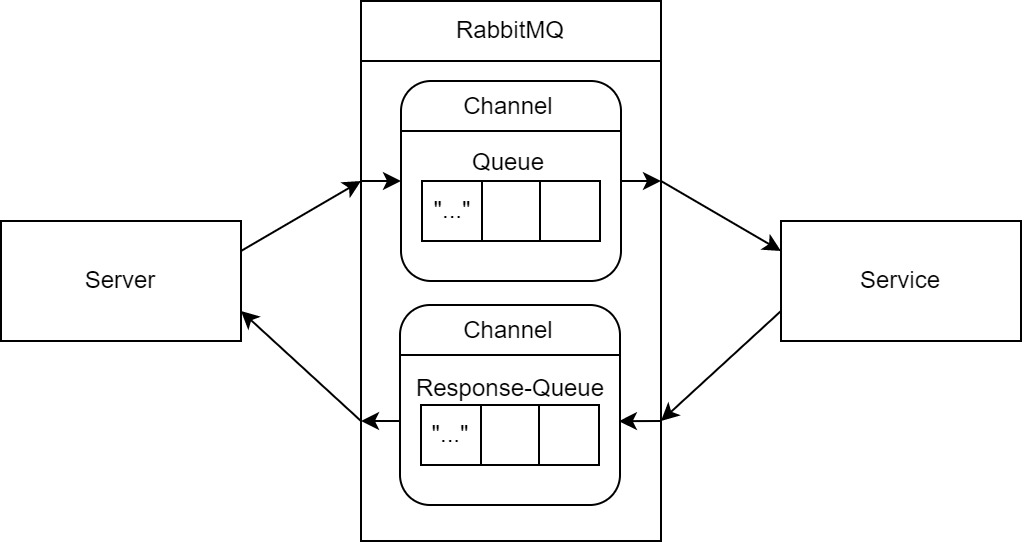
\includegraphics[width = 15cm]{bilder/Rabbit3}
    \caption{Kommunikation mit RabbitMQ}
\end{figure}

\subsubsection{Implementierung des KI-Services}
Der implementierte KI-Service lädt im ersten Schritt das KI-Modell, um mit diesem für jeden Eintrag in der Elasticsearch Datenbank einen semantischen Vektor zu generieren. Dieser semantische Vektor wird ebenfalls in der Datenbank gespeichert und kann für zukünftige abfragen genutzt werden.
Nachdem alle Einträge in der Elasticsearch Datenbank indiziert wurden, beginnt die Programmablaufschleife. Der erste Schritt der Schleife ist das Warten auf eingehende Nachrichten. Diese Nachrichten werden über RabbitMQ aus der, für den Service definierten, Queue ausgelesen. Falls keine Anfrage an den Service eingetroffen ist, wartet der Dienst auf unbestimmte Zeit. Nach dem erfolgreichen Auslesen einer Nachricht, fängt der KI-Service an, die Anfrage zu bearbeiten. Im ersten Schritt wird aus dem Satz, den der Nutzer an den Service geschickt hat, ein semantischer Vektor generiert. Dazu wird das gleiche KI-Modell wie bei der Indizierung der Einträge in der Datenbank genutzt. Daraufhin nutzt der Service den generierten Vektor und die \texttt{cosineSimilarity()} Funktion der Elasticsearch, um die semantisch ähnlichsten Texte aus der Datenbank herauszufiltern. Die Anzahl der gelieferten Ergebnisse ist abhängig von den übergebenen Parametern. Der Nutzer kann im Frontend das Key-Value Paar \texttt{search\_{}size} eingeben, welches in der Anfrage an den Service mitgeliefert wird. Sollte der Nutzer beispielsweise \texttt{\glqq search\_{}size : 3\grqq{}} eingeben, so werden die drei ähnlichsten Artikel zur gestellten Anfrage zurückgegeben. Die Ergebnisse werden in die Response Queue des Services geschrieben, damit sie im Backend weiter verarbeitet werden können. Nach erfolgreichem Durchlaufen des Prozesses, geht der Service wieder zum Zustand \glqq Auf Anfrage warten\grqq{} über. Veranschaulicht wird der Programmablauf des Services in Abbildung 13.

\begin{figure}[H]
  \centering
    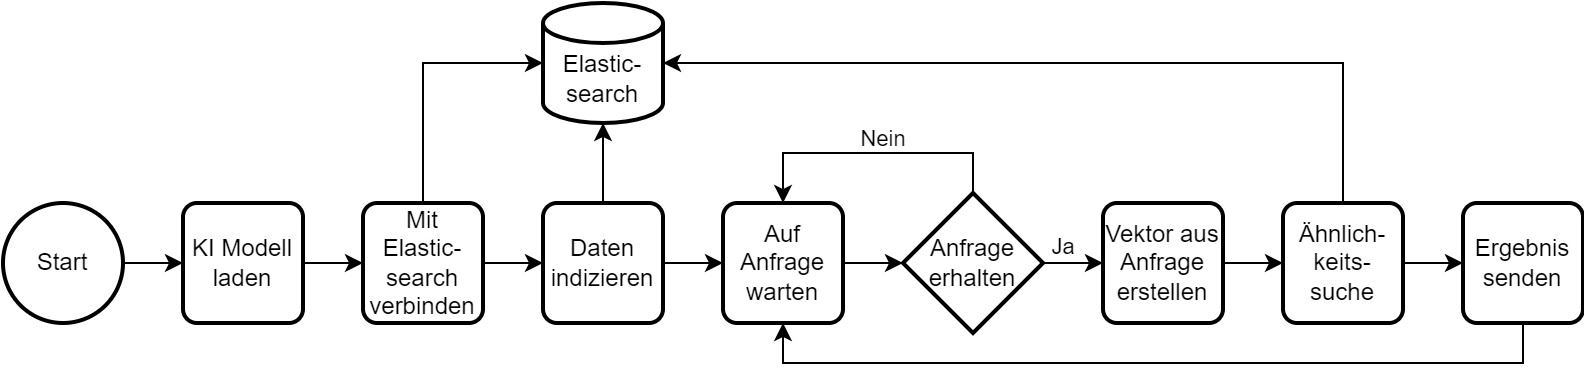
\includegraphics[width = 15cm]{bilder/KIAblauf}
    \caption{Ablaufdiagramm der Textähnlichkeitssuche}
\end{figure}

Damit der KI-Service eine Textähnlichkeitssuche durchführen kann, muss zunächst das BERT Modell importiert werden. Dieses kann der Service beim Starten automatisch aus dem offiziellen Tensorflow Hub herunterladen. Anschließen wird eine Tensorflow Session erstellt und gestartet. 

\begin{lstlisting}[language=Python, caption={Laden des BERT-Modells}]
embed = hub.Module("https://tfhub.dev/google/universal-sentence-encoder/2")
\end{lstlisting}

Im zweiten Schritt verbindet sich der Service mit der Elasticsearch-Datenbank. Dazu wird die URL, unter der die Elasticsearch erreichbar ist aus den Environment Variablen geladen. Die Environment Variablen können entweder beim manuellen Starten des Services mitgegeben werden oder falls der Service mit Docker gestartet wird, in der Docker-Compose File definiert werden. Mithilfe der URL initialisiert der Service eine Elasticsearch-Instanz und speichert sie in der Variable \texttt{client} ab. 

\begin{lstlisting}[language=Python, caption={Starten der Elasticsearch-Instanz}]
elasticsearch_url = os.environ.get('ELASTIC_URL')
client = Elasticsearch(elasticsearch_url)
\end{lstlisting}

Nachdem sich der Service erfolgreich mit der Elasticsearch verbunden hat, beginnt das Indizieren der Daten in der Datenbank. Dazu wird die Methode \texttt{index\_{}data()} aufgerufen. Der Datensatz, der für den Prototyp verwendet wurde, ist ein Auszug aus den gestellten Fragen im Forum Stackoverflow. In dem Datensatz sind 18.600 Fragen vorhanden. Jede Frage besteht aus einem Titel und einem Body. In einem Fragen-Body ist eine genauere Erläuterung der Frage, mit eventuellen Codeausschnitten oder Verlinkungen. Für die Indizierung ist lediglich der Titel der Frage genutzt worden. Das bedeutet im Umkehrschluss, dass der Titel der Frage repräsentativ für die gesamte Frage stehen muss. Nach Möglichkeit soll der Titel den gesamten Inhalt der Frage kurz und bündig zusammenfassen. Aus diesem Grund eignet  Stackoverflow sich besonders gut für den Datensatz, da in den Guidelines \glqq Write a title that summarizes the specific problem\grqq{} explizit erwähnt wird.\footcite{stackoverflow2022question}

Nach erfolgreicher Indizierung aller Fragestellungen, geht der Service in die Programmablaufschleife über. Die Schleife beginnt mit der Initialisierung der RabbitMQ Verbindung. Dort verbindet sich der der Textähnlichkeitsservice mit der Queue \texttt{text-similarity}. Bei einer eingehenden Anfrage ruft die \texttt{callback} Funktion die \texttt{respond} Funktion auf, die den KI-Algorithmus aufruft und sich um die Verarbeitung der Antwort kümmert. Die Funktion \texttt{handle\_{}query()} benötigt als Parameter die Query die vom Nutzer gestellt wurde und die Anzahl der Ergebnisse, die zurückgegeben werden sollen. Beide Parameter werden aus aus der Anfrage, die über RabbitMQ an den Service gesendet wurde, ausgelesen. Sollte es vorkommen, dass der Nutzer keine \texttt{search\_{}size} angegeben hat, wird der Standartwert 1 gesetzt.
 
\begin{lstlisting}[language=Python, caption={Auslesen der search\_{}size und Ausführen der KI}]
search_size = 1
    for p in params:
        if "search_size" in p.values():
            search_size = p["value"]

    message = handle_query(query, search_size)
\end{lstlisting}

Innerhalb der \texttt{handle\_{}query()} Methode wird zunächst der Satz, der vom Nutzer gesendet wurde, durch die Methode \texttt{embed\_{}text()} in einen Vektor konvertiert. Dieser  wird anschließend in das Feld \texttt{\glqq params\grqq{}} in der Such-Query für die Elasticsearch geschrieben. In dem Feld \texttt{\glqq source\grqq{}} wird die eigentliche Ähnlichkeitsanalyse definiert. Die Elasticsearch implementiert die Funktion \texttt{cosineSimilarity()}, die zwei Vektoren als Parameter annimmt. Der erste Vektor ist der  aus der Query zuvor generierte Vektor. Der zweite Vektor ist der aus dem Titel der Frage generierte Vektor. 

Mit der \texttt{client.search()} stellt der Service die Anfrage an die Elasticsearch mit der zuvor definierten Query. In der Anfrage wird über das Feld \texttt{\glqq size\grqq} die Anzahl der gewünschten Ergebnisse mitgeliefert. Wenn die \texttt{search\_{}size} beispielsweise 3 beträgt, werden die drei Fragen mit den ähnlichsten Vektoren in die Variable \texttt{response} geschrieben. Im nachfolgen Codesegment sind die zuvor beschriebene Erstellung des Query Vektors, der Such-Query für die Elasticsearch und die Anfrage an die Elasticsearch dargestellt.

\begin{lstlisting}[language=Python, caption={Ähnlichkeitssuche in der Elasticsearch}]
query_vector = embed_text([query])[0]
script_query = {
    [...]
        "source": "cosineSimilarity(params.query_vector, doc['title_vector']) + 1.0",
        "params": {"query_vector": query_vector}  
}
response = client.search(
    [...]
        body={
            "size": search_size,
            "query": script_query,
            [...]
        }
)
\end{lstlisting}

Die Response der Elasticsearch wird nach erfolgreicher Durchführung wieder an die \texttt{respond} Funktion übergeben. Dort wird die Nachricht vorbereitet, die als Response auf die Anfrage vom Backend zurückgesendet wird. Die Antwort wird an RabbitMQ in die Queue \texttt{response-text-similarity} gesendet.

Der Schleifendurchlauf des Services ist damit abgeschlossen. Der Service geht nun wieder, wie in Abbildung 13 zu sehen, zum Zustand \glqq Auf Anfrage warten\grqq{} über. 

\subsubsection{Management der Services}
Die entworfene Softwarearchitektur unterstützt eine beliebige Anzahl an KI-Services. Alle Services, die über das System erreichbar sein sollen, müssen über die API registriert werden. Jeder Service implementiert eine Verbindung zur RabbitMQ Schnittstelle, damit die Anfragen und Antworten asynchron zwischen dem Backend und dem jeweiligen Service gesendet werden können. Eine der Kernanforderungen für eine Architektur, die austauschbare KI-Services unterstützt, ist die dynamische Registrierung und Deregistrierung. Eine Registrierung beschreibt das Hinzufügen eines neuen Services im System, ohne den Quellcode anpassen zu müssen. Um dies zu ermöglichen, braucht es einen persistenten Speicher, in dem alle zur Verfügung stehenden Services aufgelistet sind. Zur persistenten Speicherung von kleineren Datenmengen, eignet sich eine MySQL Datenbank. Innerhalb der Datenbank werden alle aktiven Services in der Tabelle \texttt{services} abgespeichert. Zu jedem Service gibt es einen Namen mit der Bezeichnung \texttt{service} und einen Anzeigenamen mit der Bezeichnung \texttt{display\_{}name}. Der Name wird für das interne Routing über RabbitMQ genutzt. Der Anzeigename wird im Frontend innerhalb des Dropdowns für die Auswahl des Services verwendet.

\subsubsection{Automatisierte Transformation des Inputs}
Bei der Nutzung eines KI-Services kann es dazu kommen, dass die Eingaben in einer bestimmten Form vorliegen müssen. Dies ist besonders dann von Bedeutung, wenn Künstliche Intelligenzen von Drittanbietern verwendet werden. Da die Implementation oftmals als Blackbox erfolgt und nur eine Schnittstelle nach außen bereitgestellt wird, kann nicht der Algorithmus an die Daten angepasst werden, sondern die Form der Daten muss an den Algorithmus angepasst werden. Daten kommen jedoch häufiger mit überschüssigen Informationen, je nach Quelle und Methode der Datenerhebung. Die Bereinigung per Hand ist sehr aufwändig und führt schnell zu Fehlern. Sollten Echtzeitdaten an einen KI-Service angeschlossen werden, ist eine händische Bereinigung grundsätzlich nicht möglich.

Um diesem Problem entgegenzuwirken, wurde im Backend ein Algorithmus entwickelt, der Daten mithilfe einer Transformationsanleitung automatisch bereinigen kann. Die Transformationsanleitung wird durch den Anwender eingegeben und hat folgende Form:

\begin{lstlisting}[language=Python, caption={Beispiel einer Transformationsanleitung}]
{
  "seperator": "\n",
  "replace": [
    {
      "old":"\[(\d*:?)*\]",
      "new":""
    }
  ]
}
\end{lstlisting}

Aktuell im Prototyp unterstützte Transformationsoperationen sind \texttt{sperator} und \texttt{replace}. Der \texttt{sperator} teilt die vom Nutzer eingegebene Query in mehrere einzelne Queries auf. Dazu nutzt er die \texttt{split} Operation aus Python, die für Strings standardmäßig verfügbar ist. In der Transformationsanleitung wird ebenfalls ein Array an \texttt{replace} Operationen angegeben. Jeder Eintrag im \texttt{replace} Array enthält ein Objekt mit Key-Value Paaren \texttt{old} und \texttt{new}. Der alte String wird durch den neuen String ersetzt. Dazu wird die \texttt{replace} Funktion aus dem Python Package \texttt{re} verwendet. Die \texttt{replace} Funktion nutzt Regular Expression als Syntax für das Ersetzen. Dadurch sind auch komplexere Ersetzungsverfahren möglich. Im Beispiel für eine Transformationsanleitung wurde eine Regular Expression zur Entfernung eines Zeitstempels mit der Form \texttt{[12:25:10]} angegeben. Der nachfolgende Code zeigt die Implementierung der \texttt{transform} Methode, die mithilfe der Anleitung die Transformation durchführt. Zunächst wird die Query in einzelne Nachrichten geteilt. Anschließend läuft eine Schleife über alle Nachrichten und wendet alle gegebenen Transformationsschritte an. Der Algorithmus gibt ein Array an transformierten Nachrichten zurück.

\begin{lstlisting}[language=Python, caption={Transformationsalgorithmus}]
def transform(file: str, transform_json):
    [...]
    parts = file.split(transform_json['seperator'])
    messages = []
    for m in parts:
        for replacer in transform_json['replace']:
            m = re.sub(replacer['old'].replace("\\\\", "\\"), replacer['new'], m)
        m = m.strip()
        messages.append(m)
    return messages

\end{lstlisting}

\subsubsection{Fehlerbehandlung}
Während der Laufzeit des Programms kann es dazu kommen, dass im vom Nutzer produzierte Fehler auftreten. Der Nutzer kann im Bereich der Transformation syntaktisch nicht korrekte Texte eingeben, die Backend verarbeitet werden. Da Nutzereingaben ohne weitere Behandlung ebenfalls ein Sicherheitsrisiko für die Infrastruktur darstellen können, wird im Backend ein System implementiert, um die Verarbeitung der Eingaben in einer isolierten Umgebung ausführen zu können. Ähnlich wie bei der Verifizierung des JWT, ist das System zur Fehlerbehandlung auch mit Function-Wrappern und Annotations umgesetzt. 

Im Backend wird ein Exception-Handler definiert der eine Funktion mit zuvor übergebenen Parametern ausführt. Da eine fehlerhafte Ausführung auch dort zum Programmabsturz führen würde, wird die Funktion in einem try-except Block gekapselt. Alle innerhalb dieses Blocks auftretende Fehler werden abgefangen und in einem Exception Objekt gespeichert. Innerhalb des Exception Objekts ist die produzierte Fehlermeldung gespeichert. Über \texttt{str(e)} kann auf die Fehlermeldung zugegriffen werden. Innerhalb des Except Blocks wird die Fehlermeldung an den Logger weitergegeben, um diese in einer Datenbank persistent zu speichern. Nach erfolgreichem Log wird dem Frontend in einer HTTP-Response der Statuscode 500 \glqq Internal Server Error\grqq{} zurückgegeben.\footcite{fielding1999rfc2616}

\begin{lstlisting}[language=Python, caption={Exception-Handling mithilfe von Wrappern}]
[...]
 @wraps(f)
        def decorator(*args, **kwargs):
            try:
                return f(*args, **kwargs)
            except Exception as e:
                logger.log("error", f"[Server, {msg}]: {str(e)}", "none")
                return r.respond({"success": False, "error": str(e)}, status=500)
            [...]
\end{lstlisting}

Jede Funktion, die in innerhalb des Exception Handlers ausgeführt werden soll, wird mit der Annotation \texttt{@exception\_{}handler("...")} versehen. Innerhalb des Parameters wird der Ort, an dem die Funktion ausgeführt wird, und damit der Fehler auftritt, als String übergeben. Diese Information wird genutzt, um innerhalb des Fehlerlogs den Ort des Fehlers aufzulisten.

\subsubsection{Event Logging}
Das Backend implementiert ein Event Logging System mit dem Zustände und Informationen des Systems in einer Datenbank gespeichert werden können. Mithilfe von Logs können Entwickler den Ablauf eines Programms besser nachvollziehen und auftretende Fehler schneller zu ihrer Quelle zurückverfolgen. Es ist ebenfalls möglich, Systeme aufzusetzen, die die auf Logs auslesen und beim Auftreten eines Errors die zuständigen Personen alarmieren. Eine Herausforderung bei einem Logging System ist es, dass das System beim Entwickler durch das Loggen keinen erheblichen Mehraufwand produzieren soll. Im Backend wurde ein Logging System entwickelt, welches mit einer einzigen Funktion angesteuert werden kann. Die Log Funktions des Loggers wird in den verschiedenen Bereichen der Anwendung über \texttt{from logs.logger import log} importiert. Nach erfolgreichem Import, steht die \texttt{log} Funktion zur Verfügung. 

Für einen Log müssen drei Parameter übergeben werden, der Log Level, eine Message und die UUID. Die möglichen Ausdrücke für die Log Level sind in Tabelle 4 aufgeführt. Die unterstützten Log Level leiten sich aus der Funktionalität von Grafana ab, welche diese Logs mit einer zugeordneten Farbe visualisiert.

\begin{table}[H]
\centering
\begin{tabular}{c|c|c}
\textbf{Ausdruck} & \textbf{Log Level} & \textbf{Farbe}\\
\hline
emerg & critical & lila\\
fatal & critical & lila\\
alert & critical & lila\\
crit & critical & lila\\
critical & critical & lila\\
err & error & rot\\
eror & error & rot\\
error & error & rot\\
warn & warning & gelb\\
warning & warning & gelb\\
info & info & grün\\
information & info & grün\\
notice & info & grün\\
dbug & debug & blau\\
debug & debug & blau\\
trace & trace & hellblau\\
* & unknown & grau
\end{tabular}
\caption{Log Level des Event Logging Systems}
\end{table}

Innerhalb der Log Funktion wird eine Datenbank Query mit den drei Parametern und einem aktuellen Zeitstempel erstellt. Der Zeitstempel kann mithilfe des \texttt{datetime} Packages erstellt werden. Über \texttt{cursor.execute()} wird die erstellte Query in der MySQL Datenbank ausgeführt. Der Log wird als Eintrag in der Tabelle \texttt{logs} gespeichert. Im folgenden Codeausschnitt ist die Log Funktion abgebildet.

\begin{lstlisting}[language=Python, caption={Erstellung eines Logs}]
def log(level, message, uid):
    [...]
    query = f"INSERT INTO logs (`level`, `message`, `timestamp`, `uid`) VALUES (%s, %s, %s, %s)"
    cursor.execute(query, (level, message, datetime.utcnow(), str(uid)))
    [...]
\end{lstlisting}

Die produzierten Logs, die in der MySQL Datenbank hinterlegt werden, können in Grafana visualisiert werden. Dazu muss ein Dashboard angelegt werden. Innerhalb des Dashboards wird ein durch Grafana bereitgestelltes Logs Panel benötigt. Grafana ordnet alle anzuzeigenden Daten grundsätzlich nach dem Zeitpunkt der Erstellung. Innerhalb des Logs Panels wird der aktuellste Log ganz oben angezeigt. Alle anderen werden chronologisch absteigend sortiert angezeigt. Da in Grafana die MySQL Datenbank als Datenquelle hinterlegt ist, muss auch die Abfrage der Daten ist SQL stattfinden. Innerhalb der SQL Abfrage ist die Auswahl des timestamps an erster Stelle durch Grafana vorgegeben. Alle weiteren Spalten können beliebig gewählt werden. Wichtig zu beachten ist, dass eine Spalte mit dem Namen \glqq message\grqq{} direkt im Logs Panel angezeigt wird, ohne den jeweiligen Log ausklappen zu müssen. Der Name \glqq level\grqq{} ist ebenfalls von Grafana reserviert. Sollte sich der Eintrag der \glqq level\grqq{} Spalte mit einem der Ausdrücke aus Tabelle 3 decken, so wird die entsprechende Farbe für den Log genutzt. Alle weiteren selektierten Spalten werden durch Ausklappen des jeweiligen Logeintrags sichtbar. Die genutzte Query zur Abfrage der Logs ist im nachfolgenden Codesegment dargestellt.

\begin{lstlisting}[language=SQL, caption={Query zur Abfrage der Logs in Grafana}]
SELECT timestamp, message, level, uid from db_logs.logs;
\end{lstlisting}

Das Log Panel mit den aus der Query resultierenden Logs ist in Abbildung 14 abgebildet.

\begin{figure}[H]
  \centering
    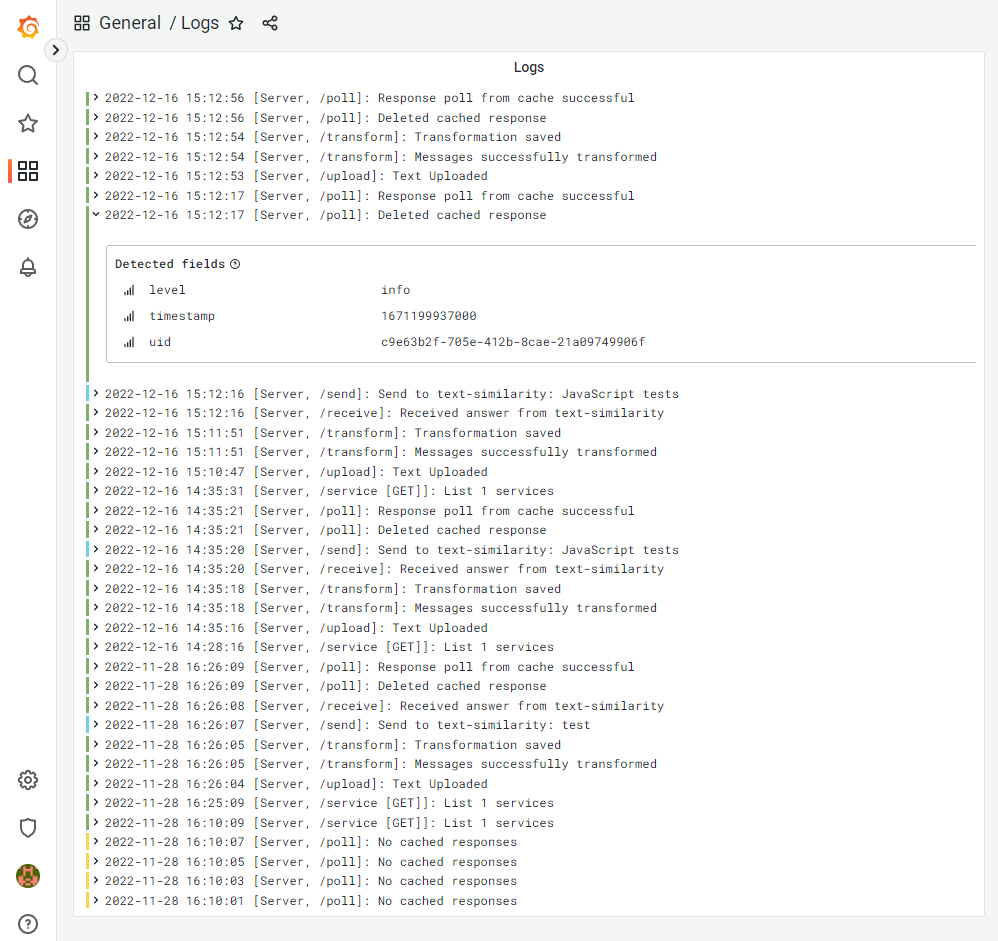
\includegraphics[width = 15cm]{bilder/grafana}
    \caption{Logs in Grafana}
\end{figure}

\subsubsection{Website mit Angular}
Damit ein Anwender die Schnittstelle zur Anbindung von Daten an KI-Services nutzen kann, wurde eine Website entworfen und entwickelt. Die grundlegende Funktionsweise der Website ist in den Abschnitten 4.1 Anforderungen und 4.2 Konzeption beschrieben. In diesem Kapitel liegt der Fokus auf der technischen Umsetzung der Website. 

Das Frontend wurde mit dem Framework Angular entwickelt. In Abbildung 15 ist der fertiggestellte Prototyp der Website dargestellt. 

\begin{figure}[H]
  \centering
    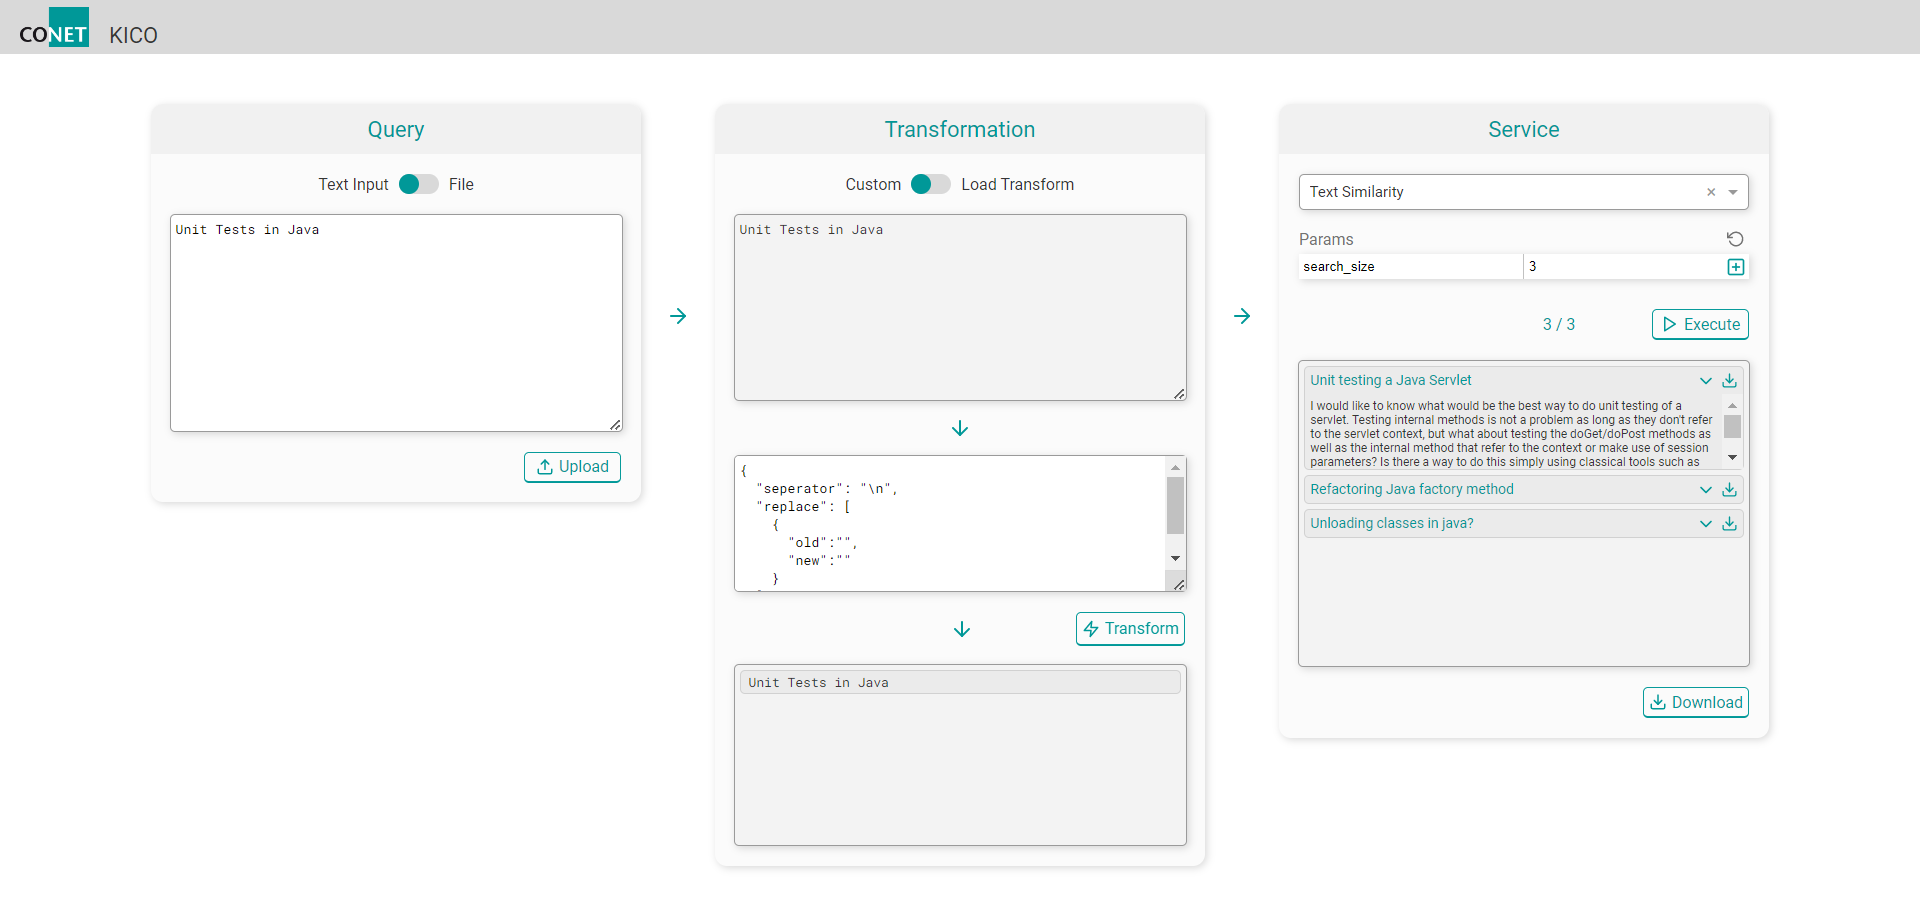
\includegraphics[width = 15cm]{bilder/website}
    \caption{Gesamtansicht der Website}
\end{figure}

Wie in den Anforderungen beschrieben, teilt sich die Website in drei Bereiche auf. In Angular ist es möglich, eigene Components zu definieren. Ein Component besteht aus drei Dateien. Die grundlegende Datei ist eine TypeScript Datei. Innerhalb dieser Datei wird der eigentliche Component definiert. Zunächst muss dafür \texttt{Component} aus \texttt{@anuglar/core} importiert werden. Im Anschluss im Bereich unter \texttt{@Component} ein selector, eine templateUrl und die styleUrls definiert. Der selector beschreibt, wie der Component im HTML Code aufgerufen werden soll. Jeder Component braucht einen individuellen Namen. Um die eigenen Components von den Components, die durch Angular bereitgestellt sind, unterscheiden zu können, befindet sich zu Beginn jedes Namens das Prefix \texttt{app-}. Die templateUrl gibt den Pfad der dazugehörigen HTML Datei an. Diese Datei ist die zweite Datei, die zur Erstellung eines Components notwendig ist. Innerhalb der styleUrls können mehrere Pfade zu verschiedenen Dateien angegeben werden. Die SCSS Datei ist die dritte Datei, die zur Erstellung eines Component benötigt wird. Im folgenden Codeausschnitt ist die Initialisierung des Query-Imput-Components innerhalb der TypeScript Datei dargestellt.

\begin{lstlisting}[language=Python, caption={Definition eines Components}]
import { Component, OnInit } from '@angular/core';

@Component({
  selector: 'app-datasource-input',
  templateUrl: './datasource.input.component.html',
  styleUrls: ['./datasource.input.component.scss']
})
\end{lstlisting}

Innerhalb der TypeScript Datei können Variablen und Funktionen definiert werden. Diese können dazu genutzt werden, Nutzerinteraktionen mit der Website festzuhalten, oder Ereignisse darzustellen. In der Query-Input-Component wird die Variable \texttt{inputStr} definiert. Innerhalb dieser Variable wird die Eingabe, die der Nutzer im Textfeld der Query-Kachel tätigt, gespeichert. Für sich alleinstehend, hat die Variable jedoch keine Funktion. Diese bekommt sie erst durch den Code aus der HTML Datei. 

\begin{lstlisting}[language=Python, caption={Erstellung einer Textarea innerhalb der HTML-Datei}]
<textarea [(ngModel)]="inputStr" placeholder="Input..." class="text-input"></textarea>
\end{lstlisting}

Innerhalb der HTML Datei für die Query ist eine Textarea definiert. Über den Selector \texttt{[(ngModel)]} kann eine Variable angegeben werden, die mit dem Inhalt der Textarea synchronisiert wird. Sobald der Nutzer eine Eingabe in der Textarea tätigt, wird diese sofort in der TypeScript Datei aktualisiert. 

Es ist ebenfalls ein \texttt{class} Attribut innerhalb der Textarea angegeben. Dieses setzt eine CSS Klasse für die Textarea. In der Definition der Component ist eine SCSS-Datei angegeben, die in diesem Schritt aufgerufen wird. Dort wird die Klasse \texttt{text-input} definiert und mit verschiedenen Style-Eigenschaften versehen. Diese Eigenschaften werden auf die Textarea angewandt.  

\begin{lstlisting}[caption={Style-Definition innerhalb einer SCSS-Datei}]
.text-input{
  border-radius: 5px;
  border: 1px solid #9A9A9A;
  box-shadow: 2px 2px 8px rgba(0,0,0,.15);
  resize: vertical;
  height: 206px;
  width: 90%;
  font-family: "Roboto Mono", sans-serif;
  padding: 5px;
}
\end{lstlisting}

Die daraus resultierende Textarea innerhalb der \glqq Query\grqq{} Kachel, ist in Abbildung 16 dargestellt.

\begin{figure}[H]
  \centering
    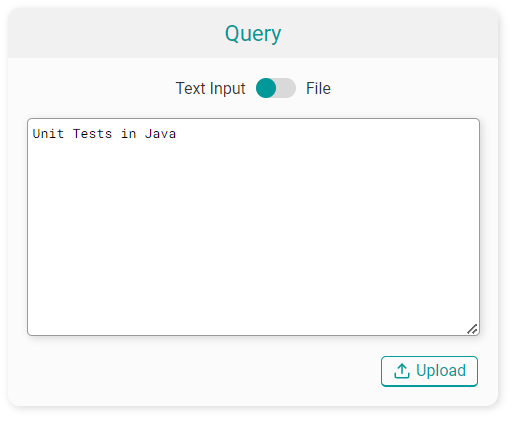
\includegraphics[width = 10cm]{bilder/websiteQuery}
    \caption{Query Kachel im Frontend}
\end{figure}

Der Bereich der Transformation besteht aus mehreren Sub-Components. Die obere und mittlere Textarea ist analog zu der Textarea aus der Query implementiert. Da die obere Textarea jedoch ausschließlich zur Bestätigung der Eingabe dient und nicht selbst zu Eingabe genutzt werden soll, wurde bei der Definition das Attribut \texttt{readonly} mitgegeben. Der untere Bereich der Transformation-Component teilt sich in zwei Components auf. Der übergeordnete Component ist das \texttt{transformation.result}. Dies ist die graue Box, in der eine Liste an transformierten Eingaben dargestellt werden. Jedes Element der Liste ist ein \texttt{transformation.result.item} Component. In Angular kann eine Liste im HTML Code direkt aus einer Variable erzeugt werden. Dazu wird \texttt{*ngFor} verwendet. Innerhalb der Schleife ist eine Variable aus der zugehörigen TypeScript Datei angegeben, über die iteriert wird. Sollte sich die Variable zur Laufzeit ändern, so wird auch direkt die HTML Datei angepasst. Der folgende Codeausschnitt zeigt die Implementierung des \texttt{transformation.result} Components.

\begin{lstlisting}[language=Python, caption={Anzeige der Results aus der Transformation}]
<div class="container">
  <li *ngFor="let item of results; index as i" class="list-results">
    <app-transformation-result-item [text]="item"></app-transformation-result-item>
  </li>
</div>
\end{lstlisting}

In Abbildung 17 ist die Transformation der Query, sowie das Ergebnis abgebildet.

\begin{figure}[H]
  \centering
    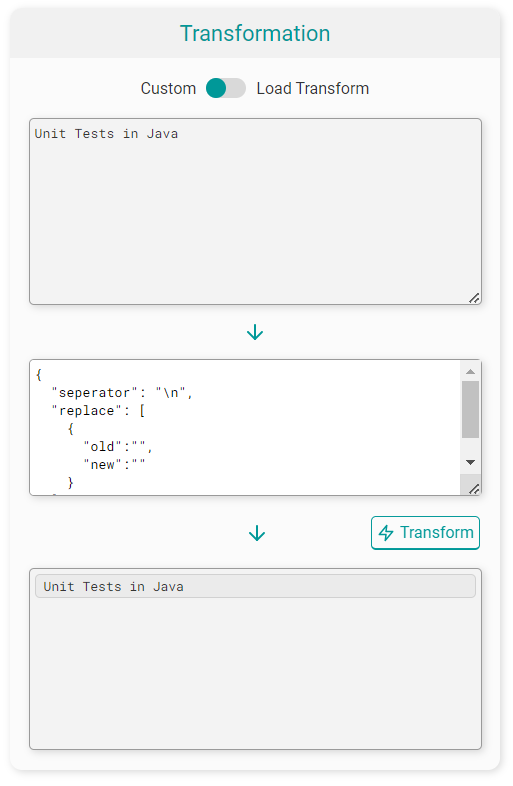
\includegraphics[width = 8cm]{bilder/websiteTransformation}
    \caption{Transformation Kachel im Frontend}
\end{figure}

Der dritte Bereich der Website stellt die Auswahl und Ergebnisauflistung des KI-Services dar. Zur Datenakquirierung werden in Angular Services verwendet. Diese sind TypeScript Dateien, die Kommunikation zur API regeln. Eine der Funktionen aus dem Service für die Service-Component ist \texttt{getService()} Methode. 

\begin{lstlisting}[language=Python, caption={Abfrage der Services}]
getServices() {
  const headers = {'Authorization': environment.token}
  return this.http.get<any>(environment.backend_url + '/service', {headers})
}
\end{lstlisting}

Diese kann innerhalb der TypeScript Datei der Component aufgerufen werden. Die \texttt{getService()} Methode stellt einen HTTP GET-Request an die \texttt{/service} Route der API. Die genaue URL der API wird aus den Environmentvariablen ausgelesen. Die Methode gibt jedoch nicht direkt die Response auf den Request zurück, sondern ein Objekt vom Typ Observable. Innerhalb des TypeScript Datei des Components kann auf dieses Observable subscribed werden. Durch diese Herangehensweise wird ein asynchroner Aufruf an die API gesendet und bei einer Response das Ergebnis verarbeitet. Das Ergebnis ist hierbei eine Liste aller verfügbaren KI-Services. Diese werden in der Variable \texttt{services} gespeichert.

\begin{lstlisting}[language=Python, caption={Subscriben auf einen Observable}]
this.serviceService.getServices().subscribe(res => {
  this.services = res['services']
})
\end{lstlisting}

Im HTML des Service-Components wird die Liste der Services für ein Dropdown verwendet. Eine weitere Funktion von Angular sind Events. Ein Event kann von einem Component ausgelöst werden. Innerhalb des Components, dass das untergeordnete Component implementiert, kann auf dieses Event reagiert werden. Es besteht die Möglichkeit TypeScript Code auszuführen oder vordefinierte Funktionen aufzurufen. Im Dropdown wird das \texttt{changeEvent} abgefangen. Dieses löst aus, wenn der Nutzer ein neues Element aus dem Dropdown ausgewählt hat. Dabei wird die Funktion \texttt{serviceSelected()} aufgerufen.

\begin{lstlisting}[language=Python, caption={Dropdown zur Auswahl der Services}]
<app-dropdown [elements]="services" (changeEvent)="serviceSelected($event)"></app-dropdown>
\end{lstlisting}

Die Tabelle für die Parameter nutzt ebenfalls \texttt{*ngFor}, um die einzelnen Reihen zu generieren. 

Der letzte Component innerhalb des Services ist der \texttt{service.result} Component. Dieser zeigt ein Ergebnis aus dem KI-Service an. Das Ergebnis besteht dabei aus einer Überschrift und einem Body. Damit die Ergebnisse beim Frontend eintreffen, muss der Nutzer nach der Auswahl des Services auf den \glqq Execute\grqq{} Button klicken. Dadurch wird im Angular Service die Methode \texttt{sendRequests()} aufgerufen, die dafür sorgt, dass die Anfrage für den KI-Service an die API gesendet wird. Anschließend wird die Funktion \texttt{pollResponses(expectedResponses: number)} mit der Anzahl der erwarteten Ergebnisse aufgerufen. Diese führt in einem 200ms Intervall die \texttt{poll()} Funktion aus, die eine Anfrage an die API stellt, ob bereits neue Ergebnisse des KI-Service im Backend zwischengespeichert wurden. Falls dies der Fall sein sollte, werden die Ergebnisse in der Response mitgeteilt und die Anzahl der erhaltenen Ergebnisse hochgezählt. Die Schleife läuft so lange, bis die Anzahl der erhaltenen Ergebnisse gleich der Anzahl der erwarteten Ergebnisse ist. Für jedes Ergebnis wird ein \texttt{service.result} Component in einer \texttt{*ngFor} Schleife erzeugt. Die Auflistung der Ergebnisse, sowie die zuvor beschriebenen Elemente der \glqq Service\grqq{} Kachel, sind in Abbildung 18 zu sehen. 

\begin{figure}[H]
  \centering
    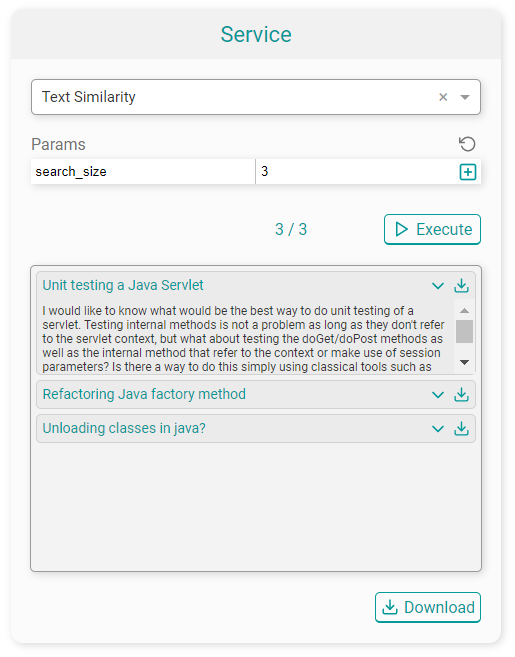
\includegraphics[width = 10cm]{bilder/websiteService}
    \caption{Service Kachel im Frontend}
\end{figure}

\subsection{Deployment der Software mit Docker}
Eine der Anforderungen der CONET war es, dass die entwickelte Schnittstelle Plattformunabhängig genutzt werden kann. Aus diesem Grund wurden alle Bereiche der Softwarearchitektur über Docker Container deploybar gemacht. Um eine eigens entwickelte Software in einen Container zu packen, muss zunächst ein Image aus der Software erstellt werden. Ein Image dient als Bauanleitung für den Container und enthält alle Dateien, die zur Ausführung des Programms benötigt werden. Ein Image kann über eine Dockerfile generiert werden. Die Dockerfile zur Erstellung des Images für das Backend ist nachfolgend abgebildet.

\begin{lstlisting}[language=Python, caption={Beispiel einer Dockefile}]
FROM python:3.10-slim
WORKDIR /app
ADD . /app
RUN pip install -r requirements.txt
EXPOSE 80
CMD ["python", "app.py"]
\end{lstlisting}

Innerhalb der Dockerfile können Pakete aus dem Dockerhub als Abhängigkeit angegeben werden, die beim Bauen des Images heruntergeladen werden. Im Falle des Backendes wird das Paket \texttt{python:3.10-slim} bezogen. Innerhalb der Dockerfile ist ebenfalls die Festlegung der Ordnerstruktur, sowie die Ausführung von Kommandos möglich.

Zum Bauen eines Images mithilfe der zuvor erstellten Dockerfile wird der \texttt{build} Befehl benötigt. Für das Backend, den KI-Service, sowie das Frontend ist eine Docker-Compose Datei zuständig. Die Docker-Compose Datei kann in einer Linux- oder \ac{wsl} Umgebung ausgeführt werden. Der dazu nötige Befehl lautet:
\begin{lstlisting}[caption={Build Befehl zur Erstellung von Docker-Images aus einer Compose-Datei}]
sudo docker compose -f '/path/to/compose/' build
\end{lstlisting}
Anschließend existieren drei Images in der Dockerumgebung, die zum Bau der Container genutzt werden können. 

\begin{lstlisting}[caption={Docker-Compose-Datei zum Bauen der Docker-Images}]
version: '3.3'
services: 
    flask-backend:
        build: 
            context: ../BA-Backend/
            network: host
    flask-services:
        build:
            context: ../BA-Services/
            network: host
    frontend:
        build:
            context: ../BA-Frontend/
            network: host
\end{lstlisting}

Der nachfolgende Auszug aus der \texttt{docker-compose.core.yml} Datei zeigt die Bauanleitung für einen Container der MySQL Datenbank. Innerhalb dieser Compose-Datei wird zunächst der Name des Services definiert. Unter diesem Namen ist der Docker Container im Netzwerk durch andere Docker Container erreichbar. Innerhalb des Services stehen mehrere Optionen zur Festlegung von Eigenschaften des Containers zur Verfügung. Über \texttt{ports} können ein oder mehrere Ports freigeschaltet werden, sodass der Container Zugriffe von außerhalb erlaubt. Im Bereich \texttt{volumes} stehen alle Ordner oder Dateien, die persistent gespeichert werden. Bei MySQL gibt es die Möglichkeit, ein initiales SQL-Skript anzugeben, welches nur bei der ersten Erstellung des Docker Containers ausgeführt wird. Das SQL-Skript erstellt eine Datenbank und die benötigten Tabellen. Im \texttt{image} Bereich ist das Image zum Bauen des Containers angegeben. Dies ist entweder ein lokal vorhandenes oder ein im Docker Hub angebotenes Image. Der letzte aufgeführte Punk \texttt{networks} beinhaltet das Netzwerk, in dem sich der Docker Container befindet. Dieses wird benötigt, damit unterschiedliche Container miteinander kommunizieren können. Dazu muss sichergestellt werden, dass alle Container im gleichen Netzwerk sind.

\begin{lstlisting}[caption={Docker-Compose-Datei zum Aufsetzen und Starten der Container}]
services:
    mysql: 
        ports: 
            - '3333:3306'
        volumes: 
            - mysql-conf:/etc/mysql/conf.d
            - mysql-storage:/var/lib/mysql
            - ./setup.sql:/docker-entrypoint-initdb.d/init.sql:r
        [...]
        image: mysql:latest
        networks:
            - custom-network
networks: 
    custom-network:
        driver: bridge
        name: custom-network
volumes:
    mysql-storage:
    mysql-conf:
\end{lstlisting}

Der Container kann mit folgendem Befehl gebaut und gestartet werden:
\begin{lstlisting}[caption={Starten eines Docker-Containers}]
sudo docker compose -f '/path/to/compose/' up -d
\end{lstlisting}

Sollte der Container anschließend wieder beendet werden, so wird folgender Befehl benötigt: 
\begin{lstlisting}[caption={Beenden eines Docker-Containers}]
sudo docker compose -f '/path/to/compose/' down
\end{lstlisting}
    \newpage
    
    \pagestyle{Evaluation}

	\section{Evaluation}
Die Evaluation der Software wurde mit einem Mitarbeiter von CONET während der Entwicklungsphase durchgeführt. Der Prototyp wurde in einem Zeitraum von sechs Wochen implementiert. Die Durchführung eines der Code-Reviews fand in regelmäßigen Abständen statt. Während des Code-Reviews wurde der derzeitige Stand der Software präsentiert, bestehende Probleme und Schwachstellen besprochen und die weiteren Entwicklungsschritte bis zum nächsten Review geplant.

\begin{itemize}[leftmargin=6em]
\item [Woche 1:] Recherche zu den Bereichen Microservice-Architekturen und Schnittstellen war die hauptsächliche Aufgabe zu Beginn des Projekts. Im ersten Code-Review wurde die geplante Architektur vorgestellt. Das primäre Feedback zur geplanten Architektur war, nicht nur eine allgemeingültige Schnittstelle zu entwickeln, sondern die Implementierung einer Textähnlichkeitssuche in den Vordergrund zu stellen. Anhand dieser KI soll die Funktionalität der Schnittstelle gezeigt werden.
\item [Woche 2:] Das Konzept für die Implementierung der Schnittstelle wurde nach einer Anpassung der geplanten Architektur entworfen. Dieses Konzept umfasst ein Architekturdiagramm, welches die Komponenten innerhalb der Software darstellt, ein Prozessablaufdiagramm, in dem die Funktionsweise und Abläufe der Schnittelle visualisiert sind und Mockups für die zu implementierende Website. Die ursprünglich geplante Kommunikation von dem Service zur API sollte ebenfalls mit RabbitMQ umgesetzt werden, statt den API-Endpunkt des Backendes zu nutzen. Dies vereinheitlicht den Programmcode und beschleunigt die Antwortzeit der KI-Services.
\item [Woche 3:] Nach Abschluss der dritten Woche, war ein Großteil der REST-API implementiert. Innerhalb dieses Code-Reviews wurde auf den Aufbau der Routen, sowie die Anbindung an die MySQL-Datenbank und den Redis-Cache geachtet. Hierzu gab es seitens CONET keine Kritik oder Verbesserungsvorschläge.
\item [Woche 4:] Während der vierten Woche wurde die API fertiggestellt und anschließend im Code-Review vorgestellt. Besonderer Fokus lag dabei auf der Implementierung des Errormanagement- und Loggingsystems. Innerhalb dieses Reviews wurde auch Grafana zur Visualisierung der Logs vorgestellt. Ein Kritikpunkt an der gewählten Kombination aus einer MySQL-Datenbank und Grafana war, dass das System bei der Anzeige einer größeren Anzahl an Logs langsam wird. Die Anzahl der angezeigten Logs in Grafana musste demnach beschränkt werden. Des Weiteren benötigt das System zum Error-Handling für den Einsatz in einer Produktivumgebung eine genauere Aufteilung der Error-Codes. Im aktuellen Zustand des Prototyps wird bei einer fehlerhaften Eingabe der Error-Code 500 zurückgegeben. Dies ist für den realen Einsatz der Anwendung allerdings nicht ausreichend.
\item [Woche 5:] In der fünften Woche wurde das Frontend entwickelt. Dabei wurde sich an den Mockups zur visuellen Gestaltung orientiert. Die Nutzung der Website war laut CONET erst mit einer kleinen Einführung verständlich. Die Website, für sich alleinstehend, bietet zu wenig Erklärungen oder Hilfestellungen, als das sie ein Unbeteiligter nutzen könnte. Die Funktionalität der Website ist jedoch gewährleistet und deckt die in den Anforderungen erhobenen Punkte ab.
\item [Woche 6:] In der letzten Woche der Entwicklungsphase wurde der KI-Service zur Textähnlichkeitssuche implementiert. Zur Kommunikation zum Backend wurde der Service an den Dienst RabbitMQ angeschlossen. Anschließend wurden die Teile der Software über Docker in einzelne Container verpackt. Dadurch konnte die Softwarearchitektur auf den Rechnern mehrerer CONET-Mitarbeiter installiert und getestet werden.
\end{itemize}

Nach dem Abschluss der Code-Reviews wurde der entwickelte Prototyp vor mehreren Mitarbeitern von CONET präsentiert. Im Anschluss an die Präsentation wurde das Ergebnis der Bachelorarbeit mit den zu Beginn erhobenen Anforderungen verglichen. Grundsätzlich erfüllt der Prototyp sämtliche Anforderungen. Die entworfene Architektur wurde für modernen, performant und skalierbar befunden. Sie bietet eine gute Grundlage, um komplexere Systeme darauf aufbauen zu können.

Es gibt jedoch, wie auch in den Code-Reviews angemerkt wurde, einige Bereiche, bei denen es Verbesserungspotential gibt. Diese betreffen jedoch ausschließlich die visuelle Aufbereitung und Nutzerinteraktion mit dem System. Die angemerkten Kritikpunkte sind folgende:

\begin{itemize}
\item Die Nutzung der Website ist nicht intuitiv für neue Nutzer
\item Grafana wird mit MySQL zu langsam für eine große Anzahl an Logs
\item Der Nutzer kann falsche Eingaben auf der Website tätigen, ohne darüber in Kenntnis gesetzt zu werden
\item Die Installation der Software ist relativ zeitaufwändig, wenn Docker nicht bereits installiert ist
\item Die Elasticsearch-Datenbank im KI-Service kann nicht mit weiteren Daten befüllt werden
\end{itemize}
  
	\newpage
	
	\pagestyle{Fazit und Ausblick}
	
    \section{Fazit und Ausblick}
\subsection{Fazit}
%\subsection{Implikation für Praxis und Forschung}
\subsection{Ausblick}
    \newpage
    
    \nocite{*}

    \printbibliography[title={Literaturverzeichnis}]
    
    %\section{Gliederung der Bachelorarbeit}
\begin{enumerate}
\item Einleitung
\item Grundlagen
\item Vorgehen im Projekt
\item Projektergebnisse
\item Fazit
\end{enumerate}
    \end{spacing}
%	\newpage
%	\begin{spacing}{1.25}
%	
%	\end{spacing}

  % \section{Anhang}\label{sec:anhang}
\begin{figure}[!ht]
    \begin{ganttchart}[vgrid,hgrid]{1}{15}
        \gantttitle{2021}{15} \\
        \gantttitle{Week}{15} \\
        \gantttitlelist{1,...,15}{1} \\
        \ganttbar{\textit{Task 1}}{1}{2} \\
        \ganttbar{\textit{Task 2}}{3}{3} \\
        \ganttbar{\textit{Task 3}}{4}{7} \\
        \ganttbar{\textit{Task 4}}{7}{7} \\
        \ganttbar{\textit{Task 5}}{8}{8} \\
        \ganttbar{\textit{Task 6}}{8}{10} \\
        \ganttbar{\textit{Task 7}}{11}{11} \\
        \ganttbar{\textit{Task 8}}{11}{11} \\
        \ganttbar{\textit{Task 9}}{11}{11} \\
        \ganttbar{\textit{Task 10}}{11}{15}
        \ganttlink{elem0}{elem1}
        \ganttlink{elem1}{elem2}
        \ganttlink{elem2}{elem3}
        \ganttlink{elem3}{elem4}
        \ganttlink{elem4}{elem5}
        \ganttlink{elem5}{elem6}
        \ganttlink{elem6}{elem7}
        \ganttlink{elem7}{elem8}
        \ganttlink{elem8}{elem9}
        \label{fig:gantchart}
    \end{ganttchart}
    \caption{Gantt-Diagramm der detaillierten Arbeitsplanung}
    \begin{itemize}
        \item \textit{Task 1:} Einarbeitung in A
        \item \textit{Task 2:} Einarbeitung in B
        \item \textit{Task 3:} Entwicklung von As
        \item \textit{Task 4:} Bewerten von A
        \item \textit{Task 5:} Entwicklung von Interviews
        \item \textit{Task 6:} Interviewen der Probanden
        \item \textit{Task 7:} Zusammenführen der Ergebnisse
        \item \textit{Task 8:} Auswertung der Ergebnisse mittels B
        \item \textit{Task 9:} Finale Auswahl des passenden A
        \item \textit{Task 10:} Schreiben der Bachelorarbeit
    \end{itemize}
\end{figure}


\end{document}